% -------------------------------------------------------------------------------------------------
%      MDSG Latex Framework
%      ============================================================================================
%      File:                  main.tex
%      Author(s):             Michael Duerr
%      Version:               1
%      Creation Date:         30. Mai 2010
%      Creation Date:         30. Mai 2010
%
%      Notes:                 - This represents the document root of this template
%                             - Binding correction is 12mm. In case you change this value, you
%                               may also need to adapt the value of \bcorlength in mdsg.sty
%                             - Switch `babel' package options `english' and `ngerman' in case
%                               your thesis is in English
%                             - if you prefer to use utf8 encoding, uncomment the corresponding
%                               line `\usepackage[utf8]{inputenc}' and comment the line
%                               `\usepackage[latin1]{inputenc}'. To compile this example you also
%                               need to include the corresponding introduction example file i.e.
%                               `introduction-UTF8.tex' or `introduction-ISO8859-1.tex'
% -------------------------------------------------------------------------------------------------
%
\documentclass[enabledeprecatedfontcommands,bibliography=totoc,listof=totoc,index=totoc,twoside=true,BCOR=12mm,DIV=12]{scrbook}
%\KOMAoptions{draft=true}                         % uncomment if you want to visualise overful hbox
%\KOMAoptions{chapterprefix=true}                 % uncomment if you like "Chapter" in front of
                                                  % chapter number
%\KOMAoptions{appendixprefix=true}                % uncomment if you like "Appendix" in front of
                                                  % appendix number
%\KOMAoptions{...}                                % feel free to add additional KOMA options
%
% =================================================================================================
% set encoding
% -------------------------------------------------------------------------------------------------
%
\usepackage[utf8]{inputenc}                       % uncomment if you prefer utf8 encoding
%\usepackage[latin1]{inputenc}                    % uncomment if you prefer latin1 encoding
%
% =================================================================================================
% load mdsg style
% -------------------------------------------------------------------------------------------------
%
%\usepackage[diplom]{mdsg}                        % uncomment the corresponding option
%\usepackage[fopra]{mdsg}
\usepackage[bachelor]{mdsg}
%\usepackage[master]{mdsg}
%
% =================================================================================================
% initialize macros
% -------------------------------------------------------------------------------------------------
%
\lmutitle{Titel der Arbeit}                       % title: you can force a new line by
%\lmutitle{Titel \\ der \\ Arbeit}                % inserting `\\'. However, this will cause
                                                  % a hyperref warning!
\lmustudentone{Tim Hesse}                         % first author's name
%\lmustudenttwo{Max2 Mustermann2}                 % second author's name
%\lmustudentthree{Max3 Mustermann3}               % third author's name
%\lmustudentfour{Max4 Mustermann4}                % fourth author's name

\lmuprofone{Prof. Dr. Claudia Linnhoff-Popien}    % first supervisor's name
%\lmuproftwo{Prof. Dr. Max Mustermann}             % second supervisor's name
                                                  % (uncomment if not needed)
%\lmuprofthree{Prof. Dr. Max2 Mustermann2}         % third supervisor's name
                                                  % (uncomment if not needed)
\lmuadvisorone{Thomas Gabor}                    % first advisor's name
\lmuadvisortwo{Thommy Phan}                    % second advisor's name
                                                  % (uncomment if not needed)
%\lmuadvisorthree{Betreuer Name3}                  % third advisor's name
                                                  % (uncomment if not needed)
\lmudraftdate{\today}                             % only for versioning during work!
                                                  % (uncomment for final version!)
\lmudeadline{15. Juli 2021}                      % deadline (day of submission)
%
% =================================================================================================
% package selection (add additional packages if needed)
% -------------------------------------------------------------------------------------------------
%
%\usepackage{layout}                              % see documentation of this package
\usepackage{cmap}                                 % to produce searchable PDF
\usepackage[T1]{fontenc}                          % split german words with umlaut
\usepackage{lmodern}
\usepackage[english]{babel}               % for german toc, ...
\usepackage{bibgerm}                              % for german bibliography index
\usepackage{tabularx}                             % more flexible table environment
\usepackage{booktabs}                             % high quality tables
\usepackage{rotating}                             % for generation of landscape tables
\usepackage{multirow}                             % for multirow cells inside tables
\usepackage{amssymb,amsmath}                      % powerful math package
\usepackage{hyperref}                             % for hyperlinks
\usepackage{fbox}
\lmuhypersetup                                    % write some pdf properties
\usepackage{flafter}                              % force floats to appear after their reference
\usepackage{subfig}                               % to allow for side by side graphics (subfloats)
\usepackage{pdflscape}                            % enable rotation of landscape pages
\usepackage{hyphenat}                             % proper hyphenation for bla_bla to bla_-bla
\usepackage[all]{hypcap}                          % correct captions
\usepackage{url}                                  % nicer url style
\usepackage{enumitem}                             % for tight lists
%\usepackage{...}                                 % add additional packages here
\usepackage[table]{xcolor-solarized}
\usepackage{wasysym}
\usepackage{textcomp}
\usepackage{listing}
\usepackage{textgreek}
\usepackage[table]{xcolor}
\usepackage{tabularx}

\setcounter{tocdepth}{3}                          % sectioning depth in toc
\setcounter{secnumdepth}{3}                       % sectioning depth in text

\graphicspath{{./pictures/}}                      % put all graphics here
% -------------------------------------------------------------------------------------------------
%      MDSG Latex Framework
%      ============================================================================================
%      File:                  hyphenation.tex
%      Author(s):             Michael Duerr
%      Version:               1
%      Creation Date:         30. Mai 2010
%      Creation Date:         30. Mai 2010
%
%      Notes:                 - Instruction \hypenation cannot handle special characters like umlaute
%                               as well as  "a and \"a. Split such words in your text.
%
% -------------------------------------------------------------------------------------------------
%
\hyphenation{Ba-che-lor-ar-}
%\hyphenation{...}                           % further hyphenation examples
                               % this file holds words latex cannot split

%
% =================================================================================================
% start of document
% -------------------------------------------------------------------------------------------------
%
\begin{document}
    \setlist{noitemsep}                           % for tight lists
    \lmufront                                     % title pages
    \newpage
    \cleardoublepage
    \lmuaffirmation                               % affirmation (work is my own work)
    \newpage
    \cleardoubleemptypage
    \thispagestyle{empty}
    % -------------------------------------------------------------------------------------------------
%      MDSG Latex Framework
%      ============================================================================================
%      File:                  abstract.tex
%      Author(s):             Michael Duerr
%      Version:               1
%      Creation Date:         30. Mai 2010
%      Creation Date:         30. Mai 2010
%
%      Notes:                 - Place your abstract here
% -------------------------------------------------------------------------------------------------
%
\vspace*{2cm}

\begin{center}
    \textbf{Abstract}
\end{center}

\vspace*{1cm}

\noindent In recent years reinforcement learning(RL) showed substantial improvement in perfect information games such
as Chess or Go compared to traditional heuristic based approaches.\\
The aim of this work was to explore the capabilities of RL in games that do not feature perfect information.
As a case study we chose the bavarian card game Schafkopf, which is a 4 player trick game that features contract
bidding, including solo and team play.
We employed the well established \textbf{Proximal Policy Optimisation} algorithm to train two agents, that use two
different approaches generating training data, to play against our own baselines(Random, Greedy, Heuristic) in a custom
\textbf{multi-agent} environment using \textbf{Python}.
By fixing the contract bidding, we were able to accurately evaluate the playing strength of our agents.
We were able to beat the Random baseline convincingly, while failing to beat the two stronger rule based players.
                       % abstract
    \thispagestyle{empty}
    \frontmatter                                  % start roman numbering
    \tableofcontents                              % toc
    \mainmatter                                   % start alpha numbering
%
% =================================================================================================
% place your document text here (take care of encoding)
% -------------------------------------------------------------------------------------------------
%
    %\input{text/introduction-UTF8}
    %% -------------------------------------------------------------------------------------------------
%      MDSG Latex Framework
%      ============================================================================================
%      File:                  introduction-[UTF8,ISO8859-1].tex
%      Author(s):             Michael Duerr
%      Version:               1
%      Creation Date:         30. Mai 2010
%      Creation Date:         30. Mai 2010
%
%      Notes:                 - Example chapter
% -------------------------------------------------------------------------------------------------
%
\chapter{Einleitung}\label{sec:Introduction}
Dies ist der \LaTeX\ Rahmen zur Bearbeitung von Bachelor-, Master-, Projekt- und Diplomarbeiten.
Alle relevanten Dateien befinden sich im Verzeichnis \verb|text|.
\section{Unterverzeichnisse und Dateien}
Das Verzeichnis \verb|text| beinhaltet weitere Unterverzeichnisse und Dateien, die den Rahmen charakterisieren.
\subsection{\textbf{main.tex}}\label{subsec:main}
Diese Datei stellt die zentrale Konfigurationsdatei f�r den Rahmen dar. Unter anderem m�ssen hier Informationen
�ber die Aufgabensteller, Betreuer, die Art der Arbeit sowie deren Title eingestellt werden.
Hier k�nnen auch weitere Pakete eingebunden werden. Die Datei ist dokumentiert und sollte selbsterkl�rend
sein.
\subsection{\textbf{hyphenation.tex}}
Manche W�rter werden von \LaTeX\ nicht (ordentlich) getrennt. Diese k�nnen in dieser Datei mit deren
Trennungsstellen hinzugef�gt werden.
\subsection{\textbf{Makefile}}
Um das Dokument zu erstellen muss man den Aufruf \verb|make all| t�tigen. Dabei werden einige tempor�re
Dateien erstellt sowie die Datei \verb|main.pdf| die das entsprechende Dokument enth�lt. Mir dem
Aufruf \verb|make clean| werden alle tempor�ren Dateien sowie die Datei \verb|main.pdf| gel�scht.
sie k�nnen die Datei \verb|Makefile| ihren Anforderungen entsprechend erweitern.
\subsection{\textbf{text}}
Es bietet sich an f�r verschiedene Kapitel eigene Quelldateien zu pflegen. Diese sollten sie alle im
Ordner \verb|text| ablegen. Wie ein Kapitel eingebunden wird, kann man aus dem Beispiel in der
Datei \verb|main.tex| ablesen. Das Verzeichnis \textbf{text} beinhaltet zudem die Datei
\verb|abstract.tex|. In diese Datei soll eine kurze Zusammenfassung (ca. eine halbe Seite)
der Arbeit eingetragen werden. Die Datei \verb|appendix.tex| kann verwendet werden um einen
Anhang zu generieren.
\subsection{\textbf{pictures}}
Hier m�ssen sie alle Grafiken ablegen, die sie in ihrem Dokument einbinden wollen. Es sind nur die
Formate PDF, PNG und JPEG erlaubt (GIF ist m�glich, wird aber nicht empfohlen).
\subsection{\textbf{bibliography.bib}}
In diese Datei m�ssen alle Referenzen eingetragen werden,
die innerhalb ihrer Arbeit zitiert werden. Verwenden sie zur Verwaltung ihrer Referenzen einen
geeigneten Editor z.B. \textit{JabRef} (\url{http://jabref.sourceforge.net/}).
\subsection{\textbf{mdsg.sty}}
Hierbei handelt es sich um das Stylefile, das das Erscheinungsbild des Dokuments
lenkt. In dieser Datei sollten in der Regel keine Ver�nderungen notwendig sein.
\section{Beispiele}
Es gibt eine Unmenge an \LaTeX\ Tutorials und Dokumentationen, die guten Einstieg in das Arbeiten mit
\LaTeX\ erm�glichen. Im Folgenden werden aber ein paar undokumentierte Minimalbeispiele gegeben, die
den direkten Einstieg erm�glichen. Betrachten sie den Quelltext, um die Beispiele nachzuvollziehen.
\subsection{Zitate}
Wir zitieren hier eine Quelle von James Aspnes et al \cite{aspn07}, die in der  Datei\\
\verb|bibliography.bib|
steht.
\subsection{Listen}
Es gibt verschiedene M�glichkeiten Listen zu erstellen, z.B. ohne Nummerierung\dots
\begin{itemize}
   \item
      Das ist der erste Punkt,
      \begin{itemize}
         \item
            das der erste Unterpunkt,
         \item
            das der zweite Unterpunkt,
   \end{itemize}
   \item
      das der zweite, und
   \item
      das der dritte Punkt.
\end{itemize}
\dots oder mit Nummerierung\dots
\begin{enumerate}
   \item
      Das ist der erste Punkt,
      \begin{enumerate}
         \item
            das der erste Unterpunkt,
         \item
            das der zweite Unterpunkt,
      \end{enumerate}
   \item
      das der zweite, und
   \item
      das der dritte Punkt.
\end{enumerate}
\subsection{Referenz auf anderen Text}
Es ist auch m�glich auf andere Stellen im Text z.B. Kapitel \ref{subsec:main} zu verweisen.
\subsection{Hoch- und tiefgestellter Text}
Man kann Text tiefstellen indem man \verb|\textsubscript| verwendet, z.B. ergibt
\begin{verbatim}
text\textsubscript{tiefgestellt}
\end{verbatim}
den Text text\textsubscript{tiefgestellt}.
Das selbe funktioniert mit \verb|\textsuperscript| verwendet, z.B. ergibt
\begin{verbatim}
text\textsuperscript{hochgestellt}
\end{verbatim}
text\textsuperscript{hochgestellt}
\subsection{Tabellen}
Es gibt sch�ne M�glichkeiten Tabellen einzubinden wie z.B. Tabelle \ref{tab:CommonParameterSettings}.
\begin{center}
\begin{table}[htbp]
{\small
\begin{center}
\begin{tabular}[center]{lrlc}
\toprule
Parameter & Value & (Unit) & Available for Chord \\
\midrule
Query timeout & 10 & seconds & $\surd$ \\
Republish timeout & 300 & seconds & $\surd$ \\ % explain this value...
Stabilize timeout & 5 & seconds & $\surd$ \\
Fix fingers timeout & 30 & seconds & $\surd$ \\
Message timeout & 1 & second & $\surd$ \\
Connect timeout & 10 & seconds & $\surd$ \\
Ping superpeer timeout & 5 & seconds & $\times$ \\
Cost-Optimality estimation timeout & 20 & seconds & $\times$ \\
Significance for change in number of superpeers & 10 & percent & $\times$ \\
Significance for change in estimations  & 10 & percent & $\times$ \\
Number of permanent superpeers & 32 & nodes & $\times$ \\
Mean number of peers & 1000 & nodes & $\surd$ \\
Mean number of lookups per hour & 60 & queries & $\surd$ \\
Mean number of shared InfoProfiles per node & 20 & & $\surd$ \\
Identifier space & 16 & bits & $\surd$ \\
Direct insertion acknowledgment & true & bool & $\times$ \\
Direct query responses & true & bool & $\times$ \\
Force query resolution & true & bool & $\surd$  \\
\bottomrule
\end{tabular}
\end{center}
} % end of tiny
\caption[Simulation parameter settings]{Common simulation parameter settings.\label{tab:CommonParameterSettings}}
\end{table}
\end{center}

\subsection{Bilder}
Man kann sehr einfach Bilder einbinden so wie z.B. in Abbildung \ref{fig:pic0}.
\begin{figure}[hpbt]
  \centering
  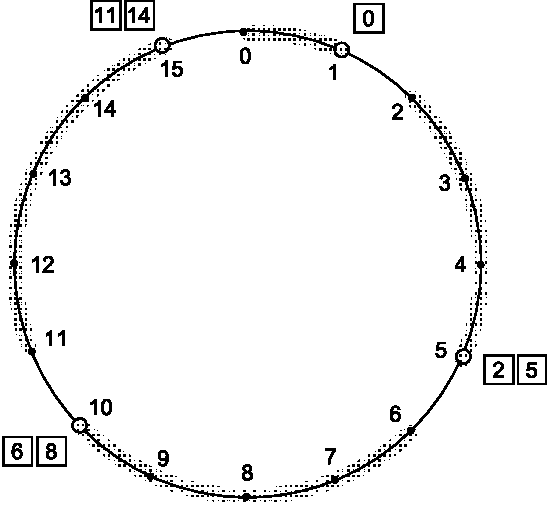
\includegraphics[width=0.4\textwidth]{pictures/pic0}\\
  \caption[Example of a $4$-bit Chord identifier circle]{Example of a $4$-bit Chord identifier circle.
  The responsibility ranges for each peer are accentuated in light gray}\label{fig:pic0}
\end{figure}
Es lassen sich auch mehrere Bilder nebeneinander platzieren wie z.B. in Abbildung
\ref{fig:multipic} zu sehen ist.
\begin{figure}[hpbt]
 \centering
  %%----start of first subfigure----
  \subfloat[FIFO size limited to 20 entries]{
   \label{fig:multipic:a} %% label for first subfigure
   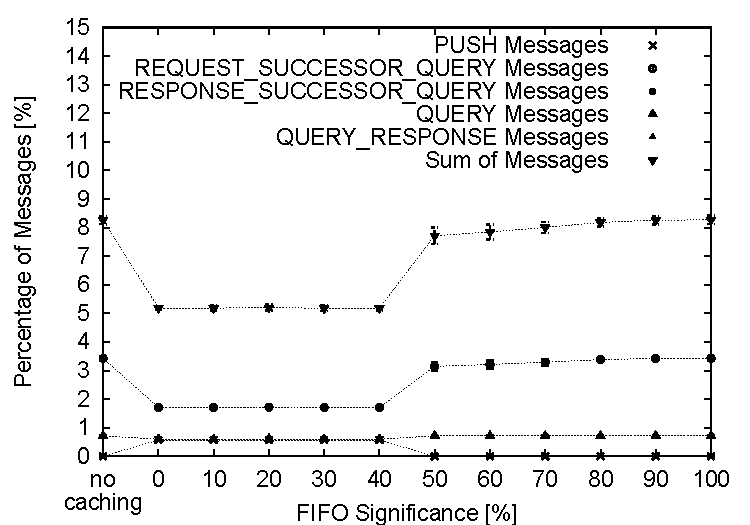
\includegraphics[width=0.48\linewidth]{pic1}}
  \hspace{0.01\textwidth}
  %%----start of second subfigure----
  \subfloat[FIFO size limited to 30 entries]{
   \label{fig:multipic:b} %% label for second subfigure
   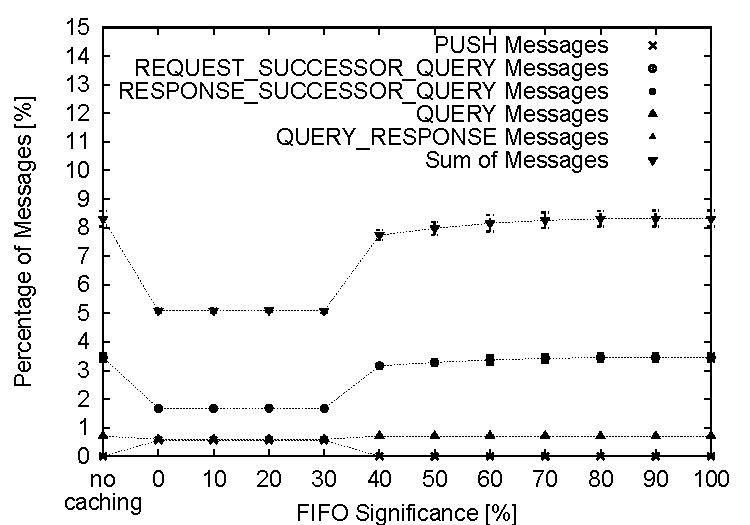
\includegraphics[width=0.48\linewidth]{pic2}}\\[0pt] % horizontal break
  %%----start of third subfigure----
  \subfloat[FIFO size limited to 40 entries]{
   \label{fig:multipic:c} %% label for third subfigure
   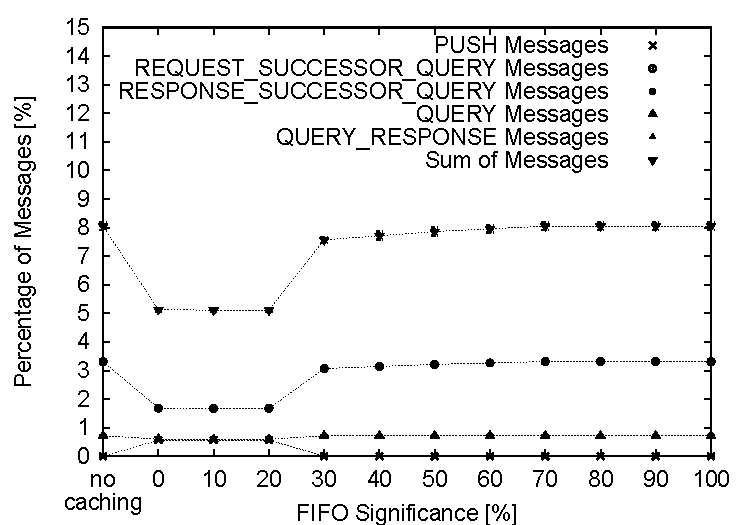
\includegraphics[width=0.48\linewidth]{pic3}}
  \hspace{0.01\textwidth}
  %%----start of fourth subfigure----
  \subfloat[FIFO size limited to 50 entries]{
   \label{fig:multipic:d} %% label for fourth subfigure
   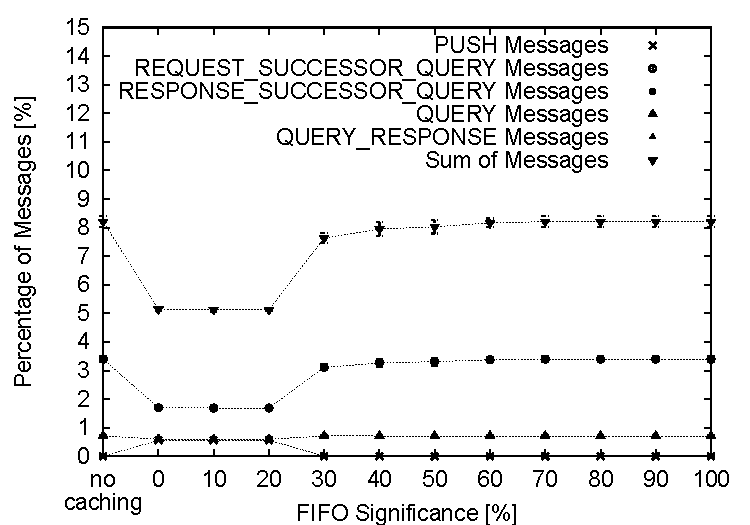
\includegraphics[width=0.48\linewidth]{pic4}}
 \caption[Observed message fractions and 95\% confidence intervals for Chord]{Observed message fractions and 95\% confidence intervals for Chord without the influence of churn. The FIFO capacity varies from 20 (\ref{fig:multipic:a}) -- 50 (\ref{fig:multipic:d}) entries (decadic steps).}
 \label{fig:multipic} %% label for entire figure
\end{figure}

\subsection{Programm Code}
Eine elegante M�glichkeit, Programmtext einzubinden, l�sst sich mit dem listings-Paket erreichen.
Das \verb|HelloWorld| Programm aus Listing \ref{lst:hw} hat in Zeile \ref{line:hw3} �brigens einen Programmierfehler.
\begin{lstlisting}[float=htp,caption=Hello World,label=lst:hw,language=Java, numbers=left, numberstyle=\tiny, stepnumber=2, numbersep=8pt, escapeinside={//@}{@//},backgroundcolor=\color{yellow},xleftmargin=3ex,xrightmargin=1ex]
public class HelloWorld {
    public static void main(String[] args) {
        Syste.out.println("Hello, World"); //@\label{line:hw3}@//
    }
}
\end{lstlisting}

\subsection{Fu�noten}
Wenn man auf Google \footnote{\url{http://www.google.com}} verweisen will, bietet sich statt einer gesonderten
Referenz auch einfach eine Fu�note an.
\subsection{Formeln}
Man kann mit \LaTeX\ sehr sch�n Formeln erzeugen:
$$L_{P}(k) = R^{orig}_{P}(k) + \sum_{i=0}^n 2*R^{i}_{P}(k)$$

    % further chapters
    \chapter{Introduction}
The application of machine learning to seemingly any problem is a constant in current literature spanning many
fields.
Improvements in processing power as well as in the algorithms used for training produced impressive results in image
recognition, protein folding, self-driving cars or robotics.\\
One domain that always lends itself to experimentation are games, since they are an enclosed domain that allow for
good evaluation and clear defined rules, and many real world problems can often be reduced and formulated as games.
\newline
Google's DeepMind showed that reinforcement learning can produce super human play in games such as Go, Chess and
Shogi.[REF]\\
These games can be classed as perfect information games as the complete state of the game is observable.
In the case of Go the possible number of game states,calculated to be around 10\textsuperscript{170} is practically
infinite[ref?], yet self play reinforcement learning algorithms in combination with Monte-Carlo-Tree-Search managed
to achieve super human play, which is a remarkable achievement in
modern times.\\
When the game state is not fully observable we speak of imperfect information games.
Card games, such as Bridge or Skat, are examples of this.
The problem is that exhaustive exploration of future possible states is of little use, since the actual game play is
heavily dependent on the cards that are dealt to each player.\\
Reinforcement learning might offer a way of through the thick fog that is imperfect information.


\section{Motivation}
Imperfect information is present in virtually every real world problem we attempt to solve with computers, so it
seems natural to test proven methods in more complex environments.
We therefore want to explore the limits of current reinforcement learning approaches for imperfect information games, as
we see this as the next achievable milestone in research.
For this we chose the bavarian card game Schafkopf to see if any reasonable playing strength can be achieved using
self-play learning and the state of the art Proximal Policy Optimisation.
It is simple enough to allow us a chance at producing good results, whilst we also have good domain knowledge, which
is beneficial for tackling hard problems such as this.
We will build an environment, baseline agents to play against and attempt at training a reasonable strong agent.


\section{Structure}
In the chapter 2[REF] we will give an overview of other people's work the field of imperfect information games, give
some background on the algorithms used.
In chapter 3 we will explain the rules of Schafkopf and show some basic strategy human players use.
Chapter 4 will explain our approach to problem. TODO
    \chapter{Rules of Schafkopf}
Schafkopf is a traditional four player trump card game that is played in the south of Germany.
The game is widely popular for being easy to learn but allowing for deep strategies.
Often it is played for small money stakes.
A game of Schafkopf normally consists of multiple rounds of four hands, where the intial dealer position rotates
clockwise around the table.
In Order to play a hand players will bid between themselves for a game contract, creating either two teams of two or
two teams of one and three, and then play 8 tricks with differing rules sets that depend on the winning bid.


\section{Cards}\label{sec:cards}
The Game of Schafkopf uses a 32 card bavarian deck, containing 4 suits with 8 ranks each.
Since the bavarian deck is comparable with a 52 french deck, where all ranks 2-6 are excluded, we also included the
corresponding English names for each suit and rank in the following tables.
The following tables is ordered descendingly by strength.
\begin{table}[]
    \begin{tabular}{lll}
        Suit     & Short Hand & Corresponding French Suit \\
        Eichel   & E          & Clubs                     \\
        Gras     & G          & Spades                    \\
        Herz     & H          & Hearts                    \\
        Schellen & S          & Diamonds
    \end{tabular}\label{tab:table2}
\end{table}
Regardless of the contract each rank has a corresponding point value ranging from 11 to 0 points in discrete steps.
The total value of all 32 cards is therefore 120.
\begin{table}[]
    \begin{tabular}{llll}
        Rank  & Point Value & Short Hand & Corresponding French Rank \\
        Ass   & 11          & A          & Ace                       \\
        Zehn  & 10          & T          & Ten                       \\
        König & 4           & K          & King                      \\
        Ober  & 3           & O          & Queen                     \\
        Unter & 2           & U          & Jack                      \\
        9     & 0           & 9          & Nine                      \\
        8     & 0           & 8          & Eight                     \\
        7     & 0           & 7          & Seven
    \end{tabular}\label{tab:table}
\end{table}
In order to refer to cards in the future we also included a short hand way of expressing suit and rank.
For example the Ten of Herz is TH and the Ober of Gras is OG.


\section{Goal and Rules}

\subsection{Goal}
The goal is to score points by taking tricks, of which there are eight.
If a team after all cards are played has 61 points (60 for the opposition) the game is won.
The rulesset for Schafkopf depends on the contract that is being played, there are however a certain rules that
always apply.

\subsection{Trumps}
Schafkopf has a set of cards that are considered trump.
This set of cards is determined by the contract that is played.
Each set has an order of strenght that always follows the order of Ober > Unter > Color.
The suits themselves have also an order of Eichel > Gras > Herz > Schellen.
As an example the order of trumps for the most common contract Team, where all Ober, all Unter and all Herz are trump:
(OE,OG,OH,OS,UE,UG,UH,US,AH,TH,KH,9H,8H,7H)

\subsection{Trick}
There are two kinds of tricks, trump and suit.
The first card of each trick,it can either be of trump or a normal suit, determines which kind is present.
In both cases players behind must play a card of that suit/trump.
If they do not possess one of that kind they may play any other card, even trump if the first card played is a suit.
\newline
A suit trick can be won either by having the highest card suit on the table or by having the highest trump on the table.
Trump tricks can however only be won by playing the highest trump.
There is no obligation to win a trick if you can do so.
Other restrictions and obligations on which cards can be played will be introduced in the Team contract section,
but the above rules are sufficient in most cases.
\section{Game Phases}
At the beginning of each player is seated at the table, and a player is randomly chosen to deal.
The initial seating relative to one another should not be changed, since the dealer position rotates after each hand
clockwise, thus
skewing the fairness.
\newline
Every hand of Schafkopf can be broken down in four distinct phases:
\begin{enumerate}
    \item Setup Phase
    \item Bidding Phase
    \item Trick Phase
    \item Scoring Phase
\end{enumerate}
To avoid complexity we excluded the doubling stage (players can choose to double the final hand reward after they
receive the first half of their hand), and the Contra stage (opposition players may double the stakes after the first card is played)
\subsection{Setup Phase}
At the beginning of a hand the player in the dealer position shuffles the cards and deals each player a hand of eight
cards.
This player is called the Dealer, and the player to his immediate left has the Lead.
\subsection{Bidding Phase}
The player with the lead starts the bidding phase and can either announce Pass or Play, then the next player clockwise announces his bid.
This continues until all players announced their intentions.
If a any previous player anounced Play, players may only also announce Play if they intend to chose a Solo Mode.
If every player passes, the hand ends and the current dealer reshuffels the cards and returns to
the Setup Phase.
If only one player announced Play, he announces his chosen contract and the Trick Phase begins.
If more than one player announced Play, the players with the highest bid wins the bid.
The order goes TEAM < WENZ < SOLO
\subsection{Trick Phase}
The player with the Lead plays his first card and the play continues in clockwise order until everybody played one
card.
The winner of the of the current trick collects all cards and becomes the new Lead.
After all eight tricks have been played the game moves into the scoring phase.
\subsection{Scoring Phase}
Each team counts their combined points, and a winner is determined.
The team that won the bid requires 61 points, whilst the opposition team only requires 60 points.
The rewards can now be calculated using a prearranged structure.
The base value of a game depends on the contract
that is being played,where SOLO modes are rewarded more due to their higher risk.
\newline
There are also specials rewards a team can earn:
\begin{description}
    \item[Schneider] The bid winners can claims Schneider when the opposition has not scored 30 points and vice versa
    if the bid winners have not scored 31 points.
    \item[Schwarz] A winning team can claim Schwarz if the other team have not won a single trick. A trick with 0
    points still counts as trick win.
    \item[Laufende] Laufende is a row of the highest trumps held by a party without interruption.
    In the TEAM game and COLOR Solo, payment is made from three Laufende (at least OE,OG,OH) and in the WENZ,
    payment is made from two Laufende (at leas UE,UG). Laufende can range from 2 up to 14 depening which contract is
    played.
\end{description}
The formula to calculate the final hand reward is always:
\begin{equation*}
    Hand Reward = Base Reward + Schneider + Schwarz + Laufende
\end{equation*}
Losers pay the winner the Hand rewards paid out always sum up to zero.
In TEAM game the losers get the negative hand reward, and the winners receive the positive hand reward.
In SOLO the bid winner receives three time the reward and each player receives a single hand reward.
The structure used in this paper can be found in the following table.
The hand is now finished, and the dealer role rotates clockwise.
\begin{table}[]
\begin{tabular}{ll}
Name     & Base Reward \\
Specials & 10          \\
Team     & 20          \\
Solo     & 50    
\end{tabular}\label{tab:table3}
\end{table}
\section{Contracts}
Schafkopf has a lot of differing contracts,these often allow for more Solo contracts or avoid aborting the hand.
All contracts follow the same trick rules we defined ealier, and only differ in the way the players are divided in
teams,what cards are Trump and the order of card ranks.
For this implementation we considered only the three classic contracts:
\begin{itemize}
    \item Team Mode
    \item Wenz
    \item Color Solo
\end{itemize}
Team mode is a two vs two variant and most, whilst WENZ and COLOR SOLO both pit the bid winner against the other three.

\subsection{Team}
In the Team game there are 14 Trumps, four Ober, four Unter and all Herz.
\newline
The bid winner calls a color ace that she does not hold herself, but she must hold at least one card of that color
that is not trump.
The player that holds the ace, being called the partner, will be allied for with the bid winner, whilst the remaining
players form the opposition team.
\newline
\begin{figure}
    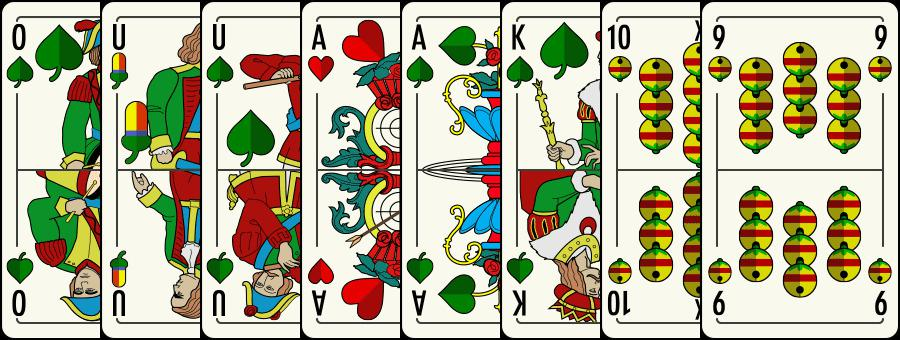
\includegraphics[scale=0.5]{partnerBiddingExample}\label{fig:figure}
    \caption{The player can only search for AS, since he holds the AG himself and has no Eichel himself}
\end{figure}
At the beginning of the hand only the partner knows the full team compositions, but in normal play this becomes
apparent fairly soon, can sometimes however last until the last trick.
If a trick starts with the searched color, the Partner has to play the ace.
This process is called Searching and reveals the team composition.
The partner may play the Ace at the beginning of a trick himself if he has the lead.
If no one searches the ace may only be played in the last trick.
If the partner has a four cards of the searched suit,including the ace, he may run away by playing a different card of
that suit, if and only if he has the lead.
Once runaway he may play the ace at any point.
This is due to the fact that if he holds 4 cards of the suit, the bid winner one, there is only one remaining cards
with the opposition.
This would guarantee a lost trick if the opposition searches and holds trump.

\subsection{Solos}
The Solos require a much stronger hand in general in order to win.

\subsubsection{Suit Solo}
The bid winner calls which color is trump.
As with the Team game there are 14 Trumps, four Ober, four Unter and six cards of the chosen color.
The team composition is obvious after the bid winner announces his game.

\subsubsection{Wenz Solo}
In the Wenz Solo the only trumps are the four Unter.
The Ober are now considered color and slot in after the King in terms of card ranking.


\section{Basic Strategy}
Schafkopf is a game with a lot of subtle and deep strategies that can take a many hands to master, yet most beginners
are given a set of base rules to follow.
Most of these rules are role dependent and will be outlined shortly below.

\subsection{Search and runaway when possible}
Players should always search when they have the chance.
Since at least two of the six searched suit cards are between the bid winner and her partner and one is with herself
the chance is high that her partner holds no cards of that suit and can trump.
The more cards of the suit he holds himself, the more likely it is that his partner is free.
Another benefit of searching is to gain information about the team composition, since the opposition knows the least
about it.\\
Due to the natural imbalance of trumps between the two teams, the oppostion will most likely score fewer tricks and
thus gains from knowing who their partner is.
This way they can use their trumps and high scoring cards more efficiently.
\newline
The searched partner in a team should always run away when he holds four suit cards in order to reduce the points lost
to the opposition.
This way he saves the 11 points of the ace for a later trick.
A rare exeption to the rule is when the searched player holds 5 cards and the bid winner the last.
In this case running away is pointless since the opposition has no means of searching in the first place.
\newline
Although this rule only applies to players that have the lead, it can still be useful in other situations.
For example when players have the chance to take the lead by winning a trick only as a means to search or run away in
the following trick.
This can sometimes mean taking away a trick of the partner or winning a low scoring trick.

\subsection{Bidder plays Trump,oppositon plays color}
This rule refers to the decision when a player has the lead, and applies to both Solo and team games.
Since the bid winner announced the game he should have more trumps than the other players and thus also fewer colors.
By playing trump when he has the lead, he can drain the opposition's trumps.
After the opposition no longer holds trump, consecutive colors such as [A,T,K] gain in strength as they cannot be
trumped anymore.
If the player had played color from the beginning, the trick could have been lost.\\
In team mode this rule also applies to the searched player and often serves as a way of signaling team membership,
since playing trump and being on the opposition in general is counterproductive.
\newline
The reverse logic applies to the opposition's strategy, as they have fewer trumps they should use the lead as an
opportunity to play color to see if they can score this way as it is unlikely to make many tricks
with trump.
If a player has aces he should play them early, before the bid winner can rid himself of that color, or play a low
color in the hope that his partner holds the ace or has trump left in case he does not hold the color himself.
\newline
In team games this strategy also servers as way of signalling team membership, especially if the lead in the first
trick opens with a suit that is not the searched ace.
By not playing trump and not searching the player signals he is part of the opposition and can not search.
His partner in turn should thus try to gain the lead in order to search before the other team drains all their trumps.

\subsection{}


    \chapter{Background}

\section{Related Work}
A common approach to treating imperfect information games (IIG) is to create a rule based player, also known as a
heuristic player.
These players often do not perform very well, even when domain experts give their insight and are often used as
baselines for evaluation.
If they are however paired with Monte-Carlo-Tree-Search(MCTS) to find strategies they can reach par-human level as
shown by Bergh et al. in 2017 for the game of Hanabi\cite{hanabi} for the game of Hanabi.\\
Monte-Carlo(MC) methods however have been the gold standard for many years.
Ginsberg used traditional Monte-Carlo sampling to build an expert Bridge player back in 2001, which shows the power
of the method \cite{gib}.\\
However even basic MC-Simulation can produce decent results with little computing power as shown by Mizukami et al.
with the popular game of Majong \cite{mahjong}.
When MCTS is extended with \textit{Upper confidence bounds} as tree policy, which is the most common approach,
human-par play can be achieved Doppelkopf \cite{Doppelkopf}, similar in many regards to Schafkopf.\\
%[ISMCTS]
For more examples and a general overview see the review from Niklaus et al. \cite{niklaus2019survey}
\newline
In terms of reinforcement learning approaches there are the results from DeepMind's Alpha Star, a self-play learning
agent for the real time strategy computer game Starcraft.
They showed how imitation learning, a method of training an initial network with games of expert players, can even find
winning strategies in an action space of 10\textsuperscript{26}. \cite{Vinyals2019}\\
Imitation learning is certainly a viable strategy, but often the data is not readily available or the quality is
lacking.
\newline
The most relevant findings to this work is the agent of Charlesworth for the game Big2, a four player card game
.\cite{Charlesworth2018}
He trained an agent using self play and the recent Proximal Policy Algorithm by OpenAI \cite{Schulman2017} and
achieved human-par play.
Interestingly he achieved his results with a significant smaller batch size compared to Bansal et al.
\cite{Bansal2017}, which trained a variety of multi-agent environments in 3D, but whether this is due to
difference in environments or other factors is unclear.
It shows at least the robustness of Proximal Policy Optimisation.


\section{Neural Networks}
Machine learning consists of three approaches to problem-solving: Supervised learning, unsupervised learning and
reinforcement learning.
We will focus on the latter one, as reinforcement learning enables agents to learn complex behaviour through
exploration within a game environment.
In this chapter I will briefly explain the key concepts and methods of reinforcement learning that allow our model
learn the game of Schafkopf.
For this we will explain neural networks, their components and internal mechanisms, the reinforcement learning approach,
Proximal Policy Optimisation, which is the training algorithm used in our experiments, and Actor-Critic models.
\newline
A \textbf{Neural Network (NN)} is an attempt to imitate the complex behaviour of the human brain that
enables us as humans to learn complex skills.
The human brain consists of billions of neurons, the basic building block inside the nervous system, that are
interconnected to form large networks, capable of processing an input signal,for example a visual stimulus, into an
output.\\

\subsection{Artificial Neuron}
To imitate this we define an artificial neuron, with the goal of creating a type of switch to process an input signal
to an output, which could again be connected to further neuron.
To do so, we give the artificial neuron an input, a weight associated with that input,an activation function and an
output.
A neuron may have multiple inputs as well as outputs and the connection between the output of one neuron to the input
of another neuron is called an edge, which in turn may have their own weights.
The output signal is calculated by passing the sum of all weighted input signals through the activation function and
can be express by the following formula:
\newline
\begin{center}
    \begin{math}
        \boxed{
            \begin{aligned}
                &\textrm{Let } k\textrm{ be the neuron }k,&\\
                &\textrm{let } n \textrm{ be the number of inputs }x,&\\
                &\textrm{let } w \textrm{ be the weight,}&\\
                &\textrm{and let }\phi \textrm{ be the activation function}&\\
                &y\textsubscript{k} = \phi (\sum_{i=0}^n w\textsubscript{kn}x\textsubscript{n})
            \end{aligned}}
        \caption{Formula to calcualate neuron output }
        \label{neuronactivation}
    \end{math}
\end{center}
There are a number of possible activation functions that can be used, but for our purpose we will look at
\textbf{Rectified Linear Unit (RELU)} and the \textbf{Softmax}.\\
\newline
\textbf{ReLU} is a simple activation function that forwards the input, if its positive, otherwise zero.
The \textbf{ReLU} function is formulated using:

\begin{center}
    \begin{math}
        \boxed{
            \begin{aligned}
                &\textrm{Let } x \textrm{ be the input of a \textbf{ReLU}}\\
                &f(x) = max(0,x)
            \end{aligned}
        }
        \caption{Definition of \textbf{ReLU} activation function}
        \label{activationRelu}
    \end{math}
\end{center}
\textbf{ReLU}, when compared to the more tradition Sigmoid activation function, has proven to be favourable in terms
of computational efficiency and performance, when applied to deep neural networks. \cite{krizhevsky2012imagenet}
For this reason we exclusively use \textbf{ReLU} in all input and hidden layers.
\\
\textbf{Softmax} is a useful activation function for output layers, as they transform any input regardless of
absolute size to an output that is within [0,1].
The output of an output layer with \textbf{Softmax} is a normalised probability distribution, where each neuron in
the layer has a probability, and the sum of all probabilities is 1.
The definition of \textbf{Softmax} is the following:
\begin{center}
    \begin{math}
        \boxed{
            \begin{aligned}
                &\textrm{Let } z \textrm{ be the vector of } N \textrm{ inputs} \\
                &f(z)_{i} = \frac{e^{z_{i}}}{\sum_{j=1}^{N} e^{z_{j}} }
            \end{aligned}
        }
        \caption{Definition of the \textbf{Softmax} activation function}
        \label{activationSoftmax}
    \end{math}
\end{center}
\newline
Now that we defined a neuron, we can use multiple neurons to form a layer, which in turn can be connected in sequence
to form a \textbf{NN}.
The minimal architecture of a network consists of three layers, whereas the middle layers are named hidden layers:
\[\text{Input layer}\Rightarrow\text{Hidden layer}\Rightarrow\text{Output layer}\]
\newline
Between adjacent layers, every neuron's input is connected to the outputs of every neuron in the previous layer and
vice versa for the following layer.
See Fig. \ref{fig:architecture} for an example.
\newline

\begin{figure}[h!]
    \centering
    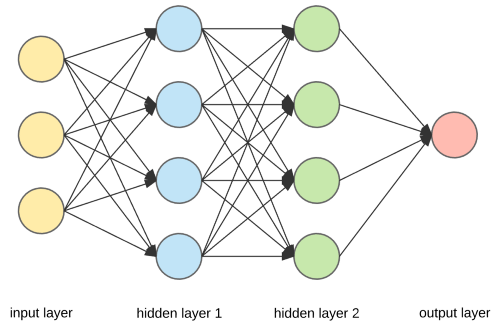
\includegraphics[scale=0.5,]{neuralnetlayer}
    \caption{Example architecture of a neural network with input,2 hidden and output layers}
    \label{fig:architecture}
\end{figure}
This kind of architecture is called \textbf{feed forward NN}, due to the process of passing an input linearly through
the network to the output, and will be used exclusively in our experiments.\\

\subsection{Policy}
The strategy for an agent to use inside an environment is called a \textbf{Policy}($\pi$).\\
The environment in our case is the game of Schafkopf, where an agent receives information about the current game
state(\textit{s}) at the time of his action that, which we use as input in our NN to make a decision on what action
(\textit{a}), in our case an action in the form of a valid card from our hand, to take.
At the end of each a hand we collect a reward(\textit{r}), which our policy over time tries to maximise.
\newline
An environment like ours can be described as \textbf{Markov Decision Process}, for which we define a four-tuple
consisting of a set states \textit{S}, a set of actions \textit{A}, a probability of our action \textit{a} as
\textit{P\textsubscript{a}} and a reward that results of that action \textit{R\textsubscript{a}}.\\
Set \textit{A} includes all the valid cards we can play in state \textit{s}.
Thus, we can define our policy as a function that takes a state and returns the probability of an action a value
function that predicts our reward \textit{r} for action \textit{a}:
\begin{center}
    \begin{math}
        \boxed{
            \begin{aligned}
                \pi(s)&\rightarrow P(a)\\
                f(s,a)&\rightarrow r_{a}\\
            \end{aligned}}
    \end{math}
\end{center}
Ideally we would want our policy to be optimal, for which we require a method of updating our NN using the
experiences and rewards we gained through interaction with the environment.
By optimal we understand, that from all states \textit{s\textsubscript{i}} we maximise the reward \textit{r}.
\newline
The process of updating a NN is called \textbf{Backpropagation}.\\
The idea is to adjust the weights of the networks neurons using a loss function, which calculates the error of our
predicted reward and our actual received reward.
Commonly used is the \textbf{Mean Square Error(MSE)}:
\begin{center}
    \begin{math}
        \boxed{
            MSE = \frac{1}{n} \sum_{i=1}^n(Y_{i}-\hat Y)^2
        }
    \end{math}
\end{center}
Ideally the \textbf{MSE} is zero, indicating that our predicted rewards are equal to the received rewards.
If not we use \textbf{Backpropagation}, which calculates the partial derivative of the total error and adjusts the
weights by traversing backwards through the NN.


\section{Actor-Critic}
The \textbf{Actor-critic} is a method of designing NNs that has a policy structure, known as the \textit{actor}
and a value structure, known as the \textit{critic}.
The \textit{actor} chooses an action for a given state, whilst the \textit{critic} evaluates the action taken.
\begin{figure}[!ht]
    \centering
    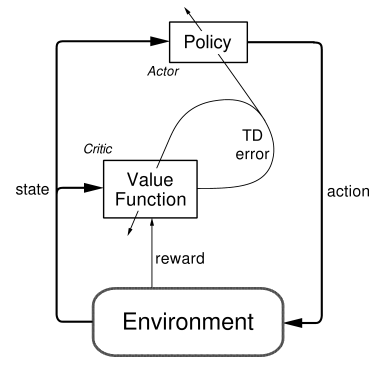
\includegraphics[scale=0.5]{actorcritic}
    \caption{Representation of an Actor-Critic model interacting with an enviroment \cite{actorcritic}}
\end{figure}


\section{Self-Play Learning}
\textbf{Self Play} learning describes the process of an agent that collects the training data itself by playing
himself, unlike in supervised learning, for which a labeled dataset needs to be provided.
The agent can figure out what works, and what does not, by stochastic exploration.
This way of generating experiences is what propelled Google's Alpha Zero to new heights and produced new strategies
modern chess engines and humans alike did not know about.\cite{Silver2017}


\section{Proximal Policy Optimisation}
\textbf{Proximal Policy Optimisation(PPO)} is a state of the art policy learning algorithm by OpenAI
.\cite{schulman2017proximal}\\
With previous algorithms it was sometimes hard to get good results due to the fact, that there were a lot of
moving parts in terms of parameter tuning of stepsizes.
If the stepsize is too low no progress is made, and vice versa one runs the risk of drowning the model in noise or
large policy updates result in a loss of progress.
Additionally, this problem is compounded by the need of tuning two cost functions for both \textit{actor} and
\textit{critic}.
\textit{PPO} solves this by introducing a trust region, that dynamically hinders the policy to make to large of a
step in either direction.
\begin{figure}[!ht]
    \centering
    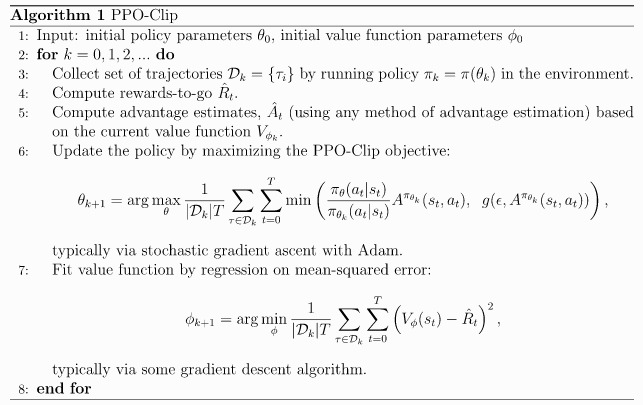
\includegraphics[scale = 0.5]{ppopseude}
    \caption{PPO-Pseudocode \cite{actorcritic}}
    \label{Pseudocode}
\end{figure}
\\
In Fig. \ref{Pseudocode} we can see in step 6 the function \textit{g}, also called the clipping function.
\begin{center}
    \begin{math}
        \boxed{
            g(\varepsilon,A) = \left\{\begin{matrix}
            (1+\varepsilon)
                                          & A \geq 0 \\
                                          (1-\varepsilon) & A < 0
            \end{matrix}\right.
        }
    \end{math}
\end{center}
If the advantage of an state-action pair is positive our policy will favour this action in the future, however only
to the extend of $\epsilon.$\\
Similary, if the advantage is negative, an action will fall out of favour in the future, but by how much is agian
limitied by $\epsilon$.
This stops our policy of making to big of change in one update step, and helps deal with noise, of which there is a
lot in stochastic games, since good decisions will not lead to good outcomes everytime.


\section{Rules of Schafkopf}
Schafkopf is a traditional four player trump card game that is played in the south of Germany.
The game is widely popular for being easy to learn but allowing for deep strategies.
Often it is played for small money stakes, but can also be enjoyed casually.
A hand of Schafkopf consist of eight tricks, and four hands make a round.
A game of Schafkopf consists therefore of multiple rounds, where the intial dealer position rotates
clockwise around the table after each hand.
In order to play a hand, players will bid between themselves for a game contract, creating either two teams of two or
two teams of one and three, and then play eight tricks with differing rules sets that depend on the winning bid.

\subsection{Cards}\label{sec:cards}
The Game of Schafkopf uses a 32 card bavarian deck, containing 4 suits with 8 ranks each.
Since the bavarian deck is comparable with a 52 french deck, where all ranks 2-6 are excluded, we also included the
corresponding English names for each suit and rank in the following tables.
The following tables is ordered descendingly by strength:
\newline
\begin{table}[h!]
    \centering
    \begin{tabular}{lll}
        \toprule
        Suit     & Short Hand & Corresponding French Suit \\
        \midrule
        Eichel   & E          & Clubs                     \\
        Gras     & G          & Spades                    \\
        Herz     & H          & Hearts                    \\
        Schellen & S          & Diamonds                  \\
        \bottomrule
    \end{tabular}
    \caption{The four suits of Schafkopf}
    \label{tab:suits}
\end{table}
\newline
Regardless of the contract each rank has a corresponding point value ranging from 11 to 0 points in discrete steps.
The total value of all 32 cards is therefore 120.
\newline
Table \ref{tab:cardsvalues} shows the order of ranks and their values.
\newline
\begin{table}[h!]
    \centering
    \begin{tabular}{llll}
        \toprule
        Rank  & Point Value & Short Hand & Corresponding French Rank \\
        \midrule
        Ass   & 11          & A          & Ace                       \\
        Zehn  & 10          & T          & Ten                       \\
        König & 4           & K          & King                      \\
        Ober  & 3           & O          & Queen                     \\
        Unter & 2           & U          & Jack                      \\
        9     & 0           & 9          & Nine                      \\
        8     & 0           & 8          & Eight                     \\
        7     & 0           & 7          & Seven                     \\
        \bottomrule
    \end{tabular}
    \caption{Card ranks of Schafkpopf and their point values}
    \label{tab:cardsvalues}
\end{table}
\newline
In order to refer to cards in the future we also included a short hand way of expressing suit and rank.
For example the Ten of Herz is TH and the Ober of Gras is OG.
A visual of all 32 cards in their traditional representation can be seen in Figure \ref{fig:32cards}
\begin{figure}[h!]
    \centering
    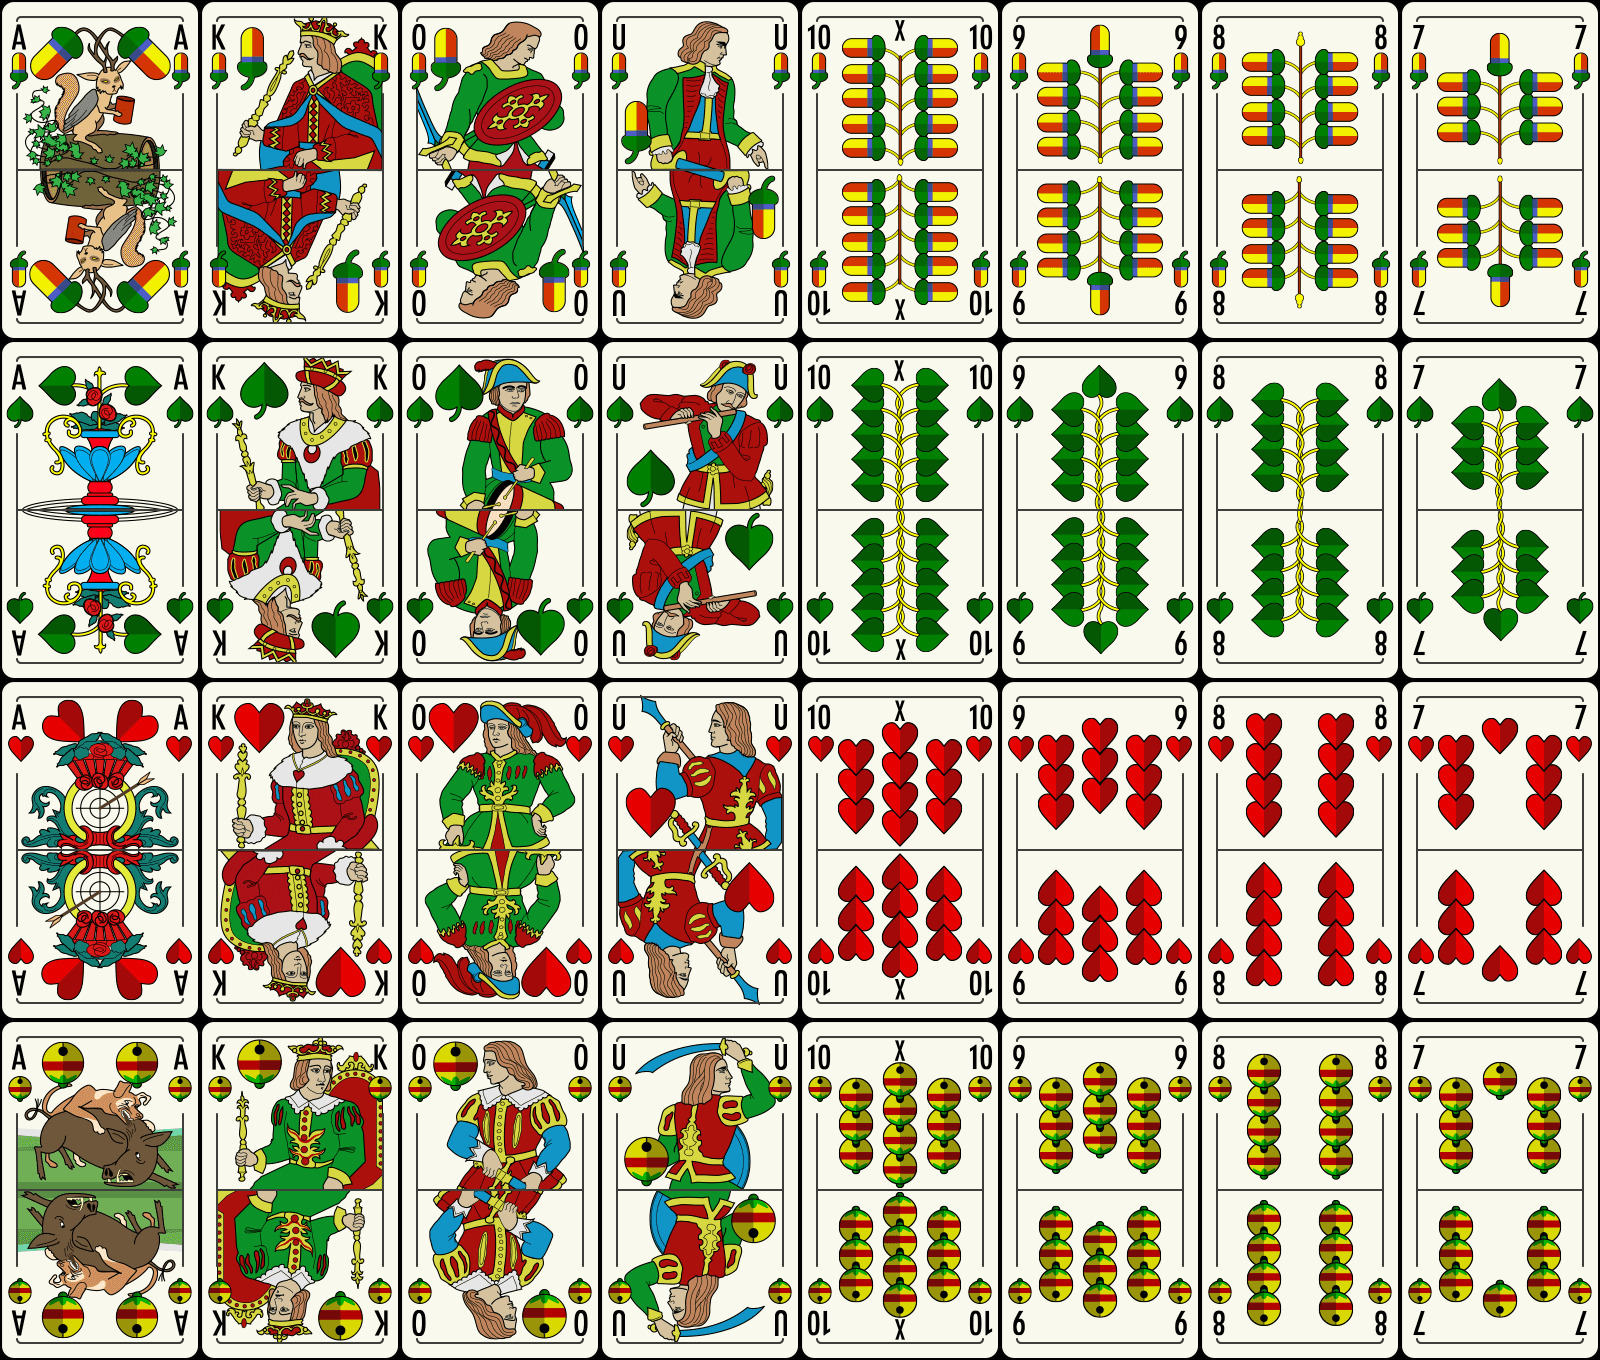
\includegraphics[scale=0.2]{cards.jpg}
    \caption{The 32 cards in Schafkopf}
    \label{fig:32cards}
\end{figure}

\subsection{Goal and Rules}

\subsubsection{Goal}
The goal is to score points by taking tricks, of which there are eight.
If a team after all cards are played has 61 points (the opposition requires only 60) the game is won.
The rules set for Schafkopf depends on the contract that is being played, there are however certain rules, such as
trick taking and following suit where possible, that always apply.

\subsubsection{Trumps}
Schafkopf has a set of cards that are considered trump.
This set of cards is determined by the contract that is played.
\newline
Each set has an order of strength that always follows the order of Ober > Unter > Color.
The suits themselves have also an order of Eichel > Gras > Herz > Schellen.
As an example the order of trumps for the most common contract Team, where all Ober, all Unter and all Herz are trump:
\newline
(OE,OG,OH,OS,UE,UG,UH,US,AH,TH,KH,9H,8H,7H)

\subsubsection{Trick}
There are two kinds of tricks, trump and suit.
The first card of each trick,which can either be of trump or a normal suit, determines which kind is present.
In both cases players behind must play a card of that suit/trump.
If they do not possess one of that kind they may play any other card, even trump if the first card played is a suit.
\newline
A suit trick can be won either by having the highest card suit on the table or by having the highest trump on the table.
Trump tricks can however only be won by playing the highest trump.
There is no obligation to win a trick if you can do so.
Other restrictions and obligations on which cards can be played will be introduced in the Team contract section,
but the above rules are sufficient in most cases.

\subsection{Game Phases}\label{gamephases}
At the beginning of each player is seated at the table, and a player is randomly chosen to deal.
The initial seating relative to one another should not be changed, since the dealer position rotates after each hand
clockwise, and if changed would skew the fairness.
\newline
Every hand of Schafkopf can be broken down in four distinct phases:
\begin{enumerate}
    \item Setup Phase
    \item Bidding Phase
    \item Trick Phase
    \item Scoring Phase
\end{enumerate}
To avoid complexity and variance we excluded, the doubling stage (players can choose to double the final hand reward
after they receive the first half of their hand), as well as the Contra stage (opposition players may double the
stakes after the first card of the first trick is played).

\subsubsection{Setup Phase}
At the beginning of a hand the player in the dealer position shuffles the cards and deals each player a hand of eight
cards.
This player is called the Dealer, and the player to his immediate left is Lead and has plays the first card in the
first trick.

\subsubsection{Bidding Phase}
The player with the lead starts the bidding phase and can either announce "Pass" or "Play", then the next player
clockwise announces his bid.
This continues until all players announced their intentions.
If a previous player announced Play, players may only also announce Play if they intend to choose a Solo Mode (Wenz
and Solo).
If every player passes, the hand ends, and the current dealer reshuffles the cards and returns to the Setup Phase.
If only one player announced Play, he announces his chosen contract, and the Trick Phase begins.
If more than one player announced "Play", the players with the higher bid wins the contract and is declared bid
winner.\\
The order goes of cotracts is: \textbf{Team < Wenz < SOLO}

\subsubsection{Trick Phase}
The player with the Lead plays his first card, and the play continues in clockwise order until everybody played one
card.
The winner of the current trick collects all cards and becomes the new Lead.
After all eight tricks have been played the game moves into the scoring phase.

\subsubsection{Scoring Phase}\label{scoringphase}
Each team counts their combined points, and a winner is determined.
The rewards can now be calculated using a prearranged structure.
The base value of a game depends on the contract
that is being played,where SOLO modes are rewarded more due to their higher risk.
\newline
There are also specials rewards a team can earn:
\begin{description}
    \item[Schneider] The bid winners can claim Schneider when the opposition has not scored 30 points and vice versa
    if the bid winners have not scored 31 points.
    \item[Schwarz] A winning team can claim Schwarz if the other team have not won a single trick.
    A trick with 0 points still counts as trick win.
    \item[Laufende] Laufende is a row of the highest trumps held by a party without interruption.
    In the Team game and COLOR Solo, payment is made from three Laufende (at least OE,OG,OH) and in the Wenz,
    payment is made from two Laufende (at leas UE,UG).
    Laufende can range from 2 up to 14 depending on which contract is played.
\end{description}
The formula to calculate the final hand reward is always:
\[\text{Hand Reward} = \text{Base Reward} + \text{Schneider} + \text{Schwarz} + \text{Laufende}\]
Losers pay the winners the Hand rewards, thus making it a zero-sum game.
In Team game the losers get the negative hand reward, and the winners receive the positive hand reward.
In SOLO the bid winner receives three time the reward and each player receives a single hand reward.
Traditionally players set a price to a reward, e.g. 1 reward point equals 0,01 \texteuro, which are eventually won or
lost.
Also the reward for different game modes may be set individually.
The structure used in this paper can be found in Table \ref{tab:rewardsStrucutre}.
After the scoring phase the hand is now finished, and the dealer role rotates clockwise to start a neew hand
\begin{table}[h!]
    \centering
    \begin{tabular}{cc}
        \toprule
        Game Mode & Base Reward \\
        \midrule
        Specials  & 10          \\
        Team      & 20          \\
        Solo      & 50          \\
        \bottomrule
    \end{tabular}
    \caption{The standard rewards in Schafkopf}
    \label{tab:rewardsStrucutre}
\end{table}

\subsection{Contracts}
Schafkopf has a lot of differing contracts, these often allow for more Solo contracts or avoid aborting the hand.
All contracts follow the same trick rules we defined earlier, and only differ in the way the players are divided in
teams,what cards are Trump and the order of card ranks.
For this implementation we considered only the three classic contracts:
\begin{itemize}
    \item Team Mode
    \item Wenz
    \item Color-Solo
\end{itemize}
Team mode is a two vs two variant and most, whilst Wenz and Color-Solo both pit the bid winner against the other three.

\subsubsection{Team}
In the Team game there are 14 Trumps: four Ober, four Unter and all Herz.
\newline
The bid winner calls a color ace that he does not hold herself, but he must hold at least one card of that color
that is not trump.
An example can be seen in Figure \ref{fig:bidding}
The player that holds the ace, being called the partner, will be allied for with the bid winner, whilst the remaining
players form the opposition team.
\newline
\begin{figure}[h!]
    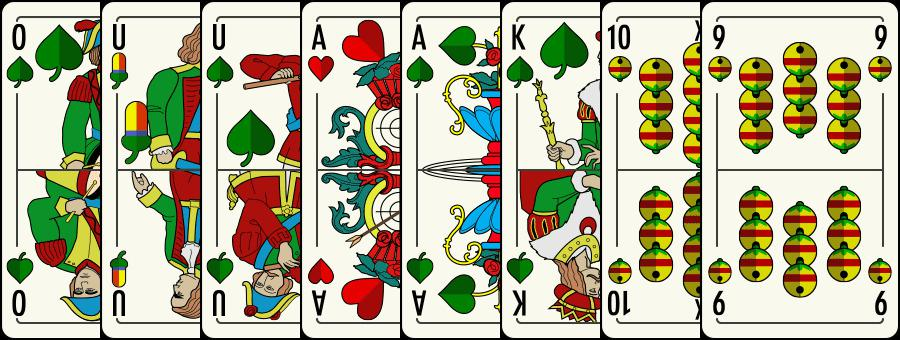
\includegraphics[scale=0.5]{partnerBiddingExample}\label{fig:figure}
    \caption{The player can only search for AS, since he holds the AG himself and has no Eichel himself}
    \label{fig:bidding}
\end{figure}
\newline
At the beginning of the hand only the partner knows the full team compositions, but in normal play this becomes
apparent fairly soon, can sometimes however last until the last trick.
If a trick starts with the searched color, the Partner has to play the ace.
This process is called Searching and reveals the team composition.
\newline
The partner may play the Ace at the beginning of a trick himself if he has the lead.
If no one searches the ace may only be played in the last trick.
If the partner has a four cards or more of the searched suit,including the ace, he may run away by playing a different
card of that suit, if and only if he has the lead.
Once runaway he may play the ace at any point.
This is due to the fact that if the partner holds 4 cards of the suit, the bid winner one, there is only one remaining
card with the opposition.
This would guarantee a lost trick if the opposition searches and holds trump.

\subsubsection{Solos}
The Solos, in which the bid winner plays alone against the other three players, require a much stronger hand in general
in order to win.
There is an obvious risk to this, due to not having a partner, but there is also a higher base reward for Solos.
This reward is also earned and lost from three players rather than one compared to the Team mode.

\subsubsection{Colour Solo}
The bid winner calls which color is trump.
As with the Team game there are 14 Trumps, four Ober, four Unter and six cards of the chosen color.
The team composition is obvious after the bid winner announces his game.

\subsubsection{Wenz Solo}
In the Wenz Solo the only trumps are the four Unter.
The Ober are now considered color and slot in after the King in terms of card ranking.


\section{Basic Strategy}\label{basicstrategy}
Schafkopf is a game with a lot of subtle and deep strategies that can take a many hands to master, yet most beginners
are given a set of base rules to follow.
Most of these rules are role dependent and will be outlined shortly below.

\subsection{Search and runaway, when possible}
Players should always search when they have the chance.
Since at least two of the six searched suit cards are between the bid winner and her partner and one is with herself
the chance is high that her partner holds no cards of that suit and can trump.
The more cards of the suit he holds himself, the more likely it is that his partner is free on the searched suit and
can win the trick by playing trump.
Often winning this trick is a requirement for the opposition to winning the game.
Another benefit of searching is to gain information about the team composition, since the opposition knows the least
about it.\\
Due to the natural imbalance of trumps between the two teams, the opposition will most likely score fewer tricks and
thus benefit from knowing who their partner is.
This way they can use their trumps and high scoring cards more efficiently.
\newline
The searched partner in a team should always run away when he holds four suit cards in order to reduce the points lost
to the opposition.
This way he saves the 11 points of the ace for a later trick.
A rare exception to the rule is when the searched player holds 5 cards and the bid winner the last.
In this case running away is pointless since the opposition has no means of searching in the first place.
\newline
Although this rule only applies to players that have the lead, it can still be useful in other situations.
For example when players have the chance to take the lead by winning a trick only as a means to search or run away in
the following trick.
This can sometimes mean taking away a trick of the partner or winning a low scoring trick.

\subsection{Bidder plays Trump, oppositon plays color}
This rule refers to the decision when a player has the lead, and applies to both Solo and team games.
Since the bid winner announced the game he should have more trumps than the other players and thus also fewer colors.
By playing trump when he has the lead, he can drain the opposition's trumps.
After the opposition no longer holds trump, consecutive colors such as [A,T,K] gain in strength as they cannot be
trumped anymore.
If the player had played color from the beginning, the trick could have been lost.\\
In team mode this rule also applies to the searched player and often serves as a way of signaling team membership,
since playing trump and being on the opposition in general is counterproductive.
\newline
The reverse logic applies to the opposition's strategy, as they have fewer trumps they should use the lead as an
opportunity to play color to see if they can score this way as it is unlikely to make many tricks
with trump.
If a player has aces he should play them early, before the bid winner can rid himself of that color, or play a low
color in the hope that his partner holds the ace or has trump left in case he does not hold the color himself.
\newline
In team games this strategy also servers as way of signalling team membership, especially if the lead in the first
trick opens with a suit that is not the searched ace.
By not playing trump and not searching the player signals he is part of the opposition and can not search.
His partner in turn should thus try to gain the lead in order to search before the other team drains all their trumps.

    \chapter{Implementation}
In this chapter we will briefly outline the approach we took for the implementation of the Schafkopf environment and
the training pipeline.


\section{Enviroment}
The environment was programmed in Python for its fast development and integration of current Reinforcement libraries
such as PyTorch, and follows the traditional Model-View-Controller(\textbf{MVC}) paradigm.
\textbf{MVC} is an established concept for game environments as it cleanly separates the game logic held in the
model
with the decision process making of the controller in our case the agents interacting with the environment.
In our implementation there are two main components necessary to play a hand of Schafkopf:
\begin{description}
    \item[Game Object] Acts as the model and handles the game logic, game phases and action validation
    \item[Player Object] Acts as the controller and makes an agents individual decision based on the implemented logic
\end{description}

\subsection{Game Object}
The game object is initialised with a list of four agent objects, a lead variable that determines the player position
with the \textbf{Lead} role.
Optionally a seed variable can be passed to control
Internally it follows the game phases defined in \ref{gamephases} .\\
In the\textbf{ Setup phase} it creates a shuffled 32 card deck and deals each player eight cards.
The deck's order can optionally be controlled via a seed variable, which can be useful for debugging or replaying
certain games for evaluation, for example if we want only seeds that give players \textbf{Solo} cards.
\newline
During \textbf{Bidding phase} each player in their respective order at the virtual table is given their hand in
combination with their valid bidding options, which depend on previous bids as well as their hand, by calling the
players' bidding methods.
Once every player has returned their bid the \textbf{Bidding phase} concludes, the highest bid and resulting game
mode can be
determined.
If at this stage no contract has been decided the hand ends immediately.
The hand moves now into the \textbf{Trick phase} after variables such as team composition, run away possibilities and
other game mode induced variables have been evaluated.
\newline
In \textbf{Trick phase} for each of the eight tricks we perform the same loop of actions starting with the leading
player:
\begin{enumerate}
    \item Set the players current hand in the corresponding player object
    \item Determine the valid cards the player may play
    \item Pass the game state,current trick history and valid cards to player by calling player's \textit{playCard}
    method
    \item Check if the action returned by the player is valid
\end{enumerate}
After all players played their card, the trick winner is determined, the point scores are updated, and played cards
are removed from the corresponding hands.
After \textbf{Team Mode} it is also important to check if players \textbf{ran away} or \textbf{searched} as this is
vital to allow for correct deduction of valid cards that can be played.
\newline
Once all eight tricks have been played successfully the \textbf{Scoring phase} commences and a winner and resulting
reward is calculated and the hand is concluded.
\subsection{Game State}
The game state holds all information that define a hand at any moment and is held and passed as dictionary throughout
the environment.
\newline
\begin{table}[h!]
\begin{tabular}{lll}
Name              & Type           & Description                                                             \\
\hline
Hands             & List of Cards  & Description                                                             \\
Game Mode         & Category       & Can be one of eigth possible contracts                                  \\
Lead              & Int            & Table position of leading player                                        \\
Scores            & List of Int    & List of length four                                                     \\
Trick History     & Tuple of Cards & Tuples that keep track of pass tricks                                   \\
Cards Played      & List of Cards  & List of all the cards played (Not necessary, but useful for perfomance) \\
Seed              & Int            & Records the Seed for debugging and evaluation                           \\
Offensive Players & Int            & List of table positions of bid winner and partner                       \\
Run Away Possible & Bool           & Can partner technically run away                                        \\
Ran Away          & Bool           & Did partner run away                                                    \\
Searched          & Bool           & Has been searched
\end{tabular}
\caption{Game state and its members.}
\label{tab:gamestate}
\end{table}

\subsection{Player Class}
The player class is a template class \ref{lst:playerclass} that every agent inherits from.
It handles an agent's decision process during the bidding phase as well as the trick phase.
The two main methods that any agent has to shadow are \textit{makebid()} and \textit{playCard()}.
These are called by the environment and make the agent the controller in the \textbf{MVC} paradigm.
\newline
\begin{lstlisting}[language=Python,label={lst:playerclass}]
import random
class Player():
    def __init__(self, name):
        self.name = name
        self.hand = []
        self.position = None

    def setHand(self, cards):
        self.hand = []
        self.hand = cards

    def setPosition(self, postion):
        self.position = postion

    def makeBid(self, validBids):
        return random.choice(validBids)

    def playCard(self, validCards, gameState, trickHistory):
        return random.choice(validCards)
\end{lstlisting}
\section{Reinforcement Learning Setup}
The common reinforcement learning libraries(OpenAI and RLlib) either did either not support multi-agent learning
environments or turn-based game types, so we decided on implementing the learning setup in PyTorch.
The actual training was performed on Google Colab, even though our training was not very GPU intensive, it proved
useful to avoid crashing local machines on long training runs with large batch sizes.
\subsection{PPO}
The \textbf{PPO} implementation used was taken and adapted from a similar project on GitHub \cite{emerich}
This allowed to set hyper-paramaters, such as learning rate, clipping values, decay, batch size.
\subsection{One-Hot Encoding}
To encode the game state into a vector we encoded all necessary information using One-hot encoding.
Cards and hands were encoded using a 32 bit vector, where each index represents a unique card.\\
The index of a card can be calculated using \[index(card) = Suit * 8 + rank\].
When positions are passed they are always a 4 bit vector where index 0 is the player.
This way all information, like bid winner and current lead, is always from the ego perspective.
\subsection{Player experiences}
To update our network we need to collect the experiences of each player during their exploration of the game
environment.
We collect at each step in the hand:
\begin{description}
\item[Action] The sampled action that was taken
\item[Log Probabilities] The probability distribution of our action space
\item[State] The input state
\item[Terminal] True if the action was terminal (last trick), otherwise False
\item[Reward] Final Reward of the hand
\end{description}
Due to the nature of Schafkopf, rewards are only received at the end of each episode.
We use reward discounting to assign rewards to non-terminal states as well by multiplying the terminal reward with a
discount factor (0.99 was used). See the code below for the method used.
\begin{lstlisting}[language=Python,label={lst:rewards},caption={Reward calculation for non-terminal steps}]
rewards = []
gamma = 0.99
discountedReward = 0
for reward, isTerminal in zip(rewards), terminal)):
if isTerminal:
discountedReward = 0
discountedReward = reward + (self.gamma * discountedReward)
rewards.append(discountedReward)
\end{lstlisting}
With this we can create for each hand eight Markov decision tuples: \[(S,A,P_{a},R_{a})\]\\
These make up our training data for our PPO update.
Since we use self play with four identical agents we actually get 32 tuples for each hand we play during self-play.

\subsection{Training Pipeline}
The training pipe line always follows the same procedure for each episode:
\begin{enumerate}
\item Load the latest model
\item Play hands with
\item Collect Experiences from each player
\item Update the network using PPO
\item Run evaluation against baseline agents
\item Log results for evaluation and for update
\item Save the updated network
\end{enumerate}



\section{Reinforcement Learning Agents}
The models we trained are simple {\textbf{feed forward NN} that receive a game state, which is processed and then fed
through the Network to produce two outputs: 32x1 vector that gives us our probabilities of all the valid
actions (\textit{actor}), and 1x1 vector which describes our state-value function (\textit{critic}). (See Fig
.\ref{fig:layerchart})\\
All inner layers use 48 hidden \textbf{ReLÚ} neurons
Overall we trained two agents, \textbf{CompleteRL} and \textbf{SeperatedRL}, that both use the same actor-critc network
design.
\begin{figure}[!h]
\centering
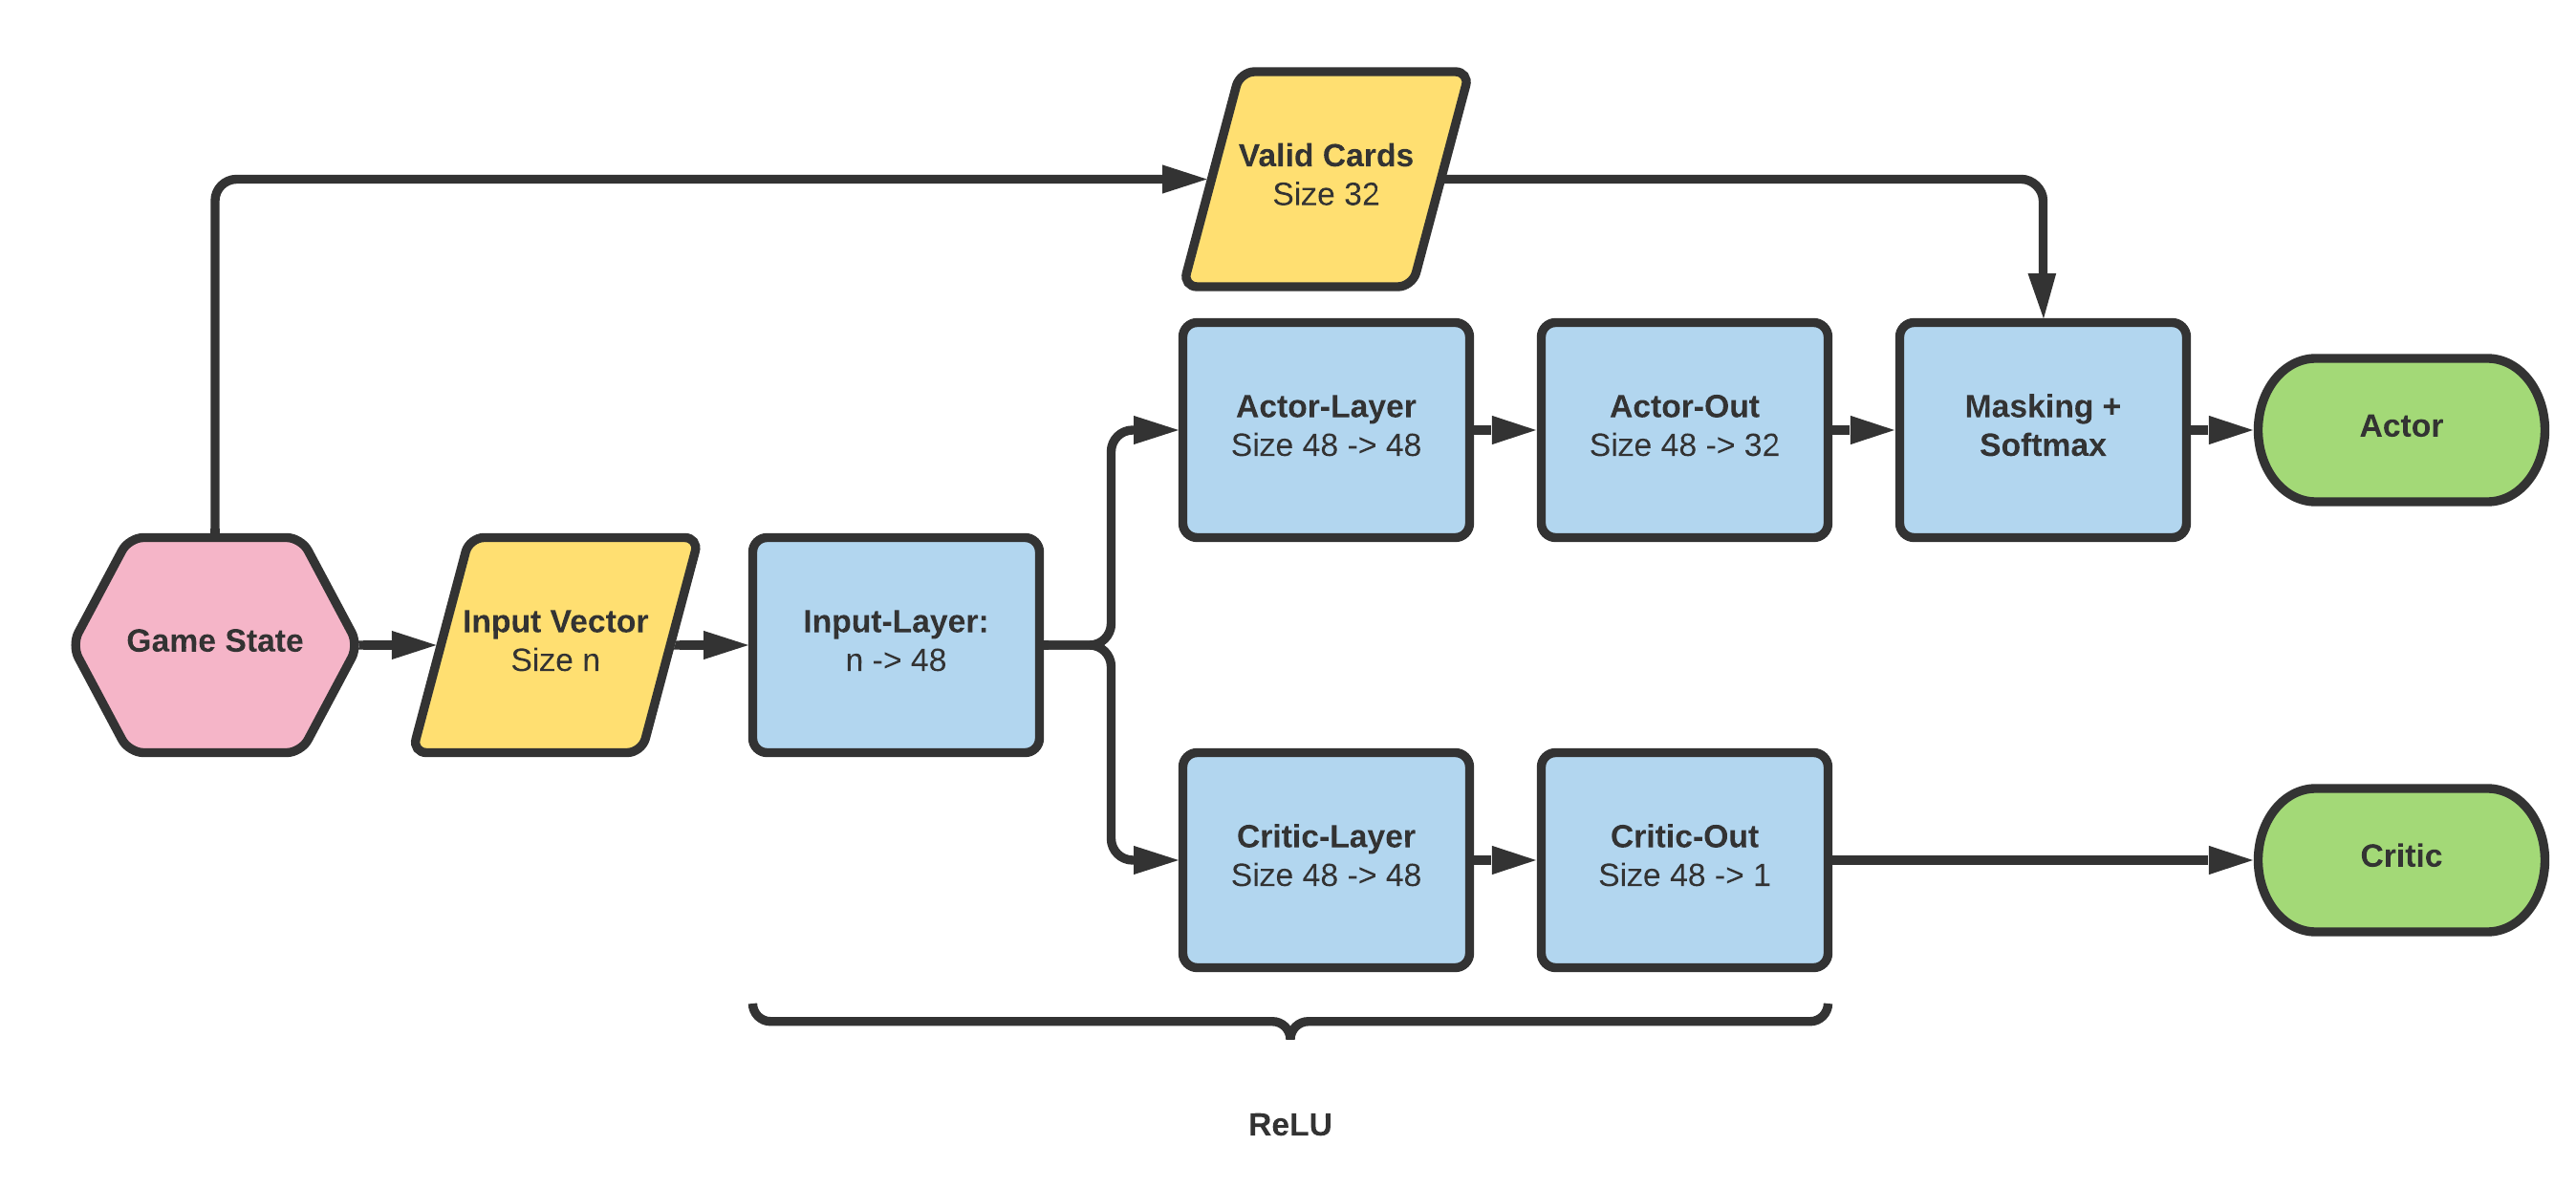
\includegraphics[width=\textwidth]{layerchart.png}
\caption{Network layer flow used the Actor-Critic Models}
\label{fig:layerchart}
\end{figure}
\subsection{CompleteRL}
The CompleteRL agent uses the same network for all three game modes.
This was our initial approach, to see if one network can do it all.
The input vector (See Tab. \ref{tab:completerlinput}), derived from the game state, uses \textit{one hot encoding}
for all cards, positions and information and is always rotated so the acting player is in position zero, to keep the
vector representation
consistent.\\
\begin{table}[!h]
\centering
\begin{tabular}{lll}
\toprule
Name          & Size     & Description                                           \\
\midrule
Hand          & 32       & Hand of the player                                    \\
Cards Played  & 32       & All cards in previous tricks                          \\
Lead          & 4        & Position that started the trick                       \\
Game Mode     & 7        & 3 contracts + 4 colours                               \\
Ran Away      & 1        & If partner ran away (Bool)                            \\
Searched      & 1        & If the ace has been searched (Bool)                   \\
Bid Winner    & 4        & Position that won the bidding                         \\
Own Team      & 4        & Position of own Team (1000 if unknown)                \\
Scores        & \(4*1\)      & Scores for each position (Normalised using Score/120) \\
Trick History & \((32+4)*4\) & Cards played by each position                        \\
\midrule
Sum & 233 & Total size of the input Vector\\
\bottomrule
\end{tabular}
\label{tab:completerlinput}
\caption{Input vector for the CompleteRL model}

\end{table}

\subsection{SeperatedRL}
As an experiment we also trained \textbf{SeperatedRL} that has a different model for each of the three contracts
(Team,Wenz,Solo).
The idea is to reduce the variance in the training data, whilst also only including the relevant information and thus
slimming the input vector.
The major drawback of this is naturally training time, but we reduced the batch size during training compared to
\textbf{SeperatedRL}.

\begin{table}[!h]
    \centering
    \begin{tabular}{lllll}
        \toprule
        Name & \multicolumn{3}{c}{Size} & Description
        \\
        \midrule
        & Team & Wenz & Colour-Solo &
        \\
\midrule
Hand          & 32       & 32                        & 32                              & Hand of the player
\\
Cards Played  & 32       & 32                        & 32                              & All cards in previous tricks
\\
Lead          & 4        & 4                         & 4                               & Position that started the
trick                       \\
Game Mode     & 4        & 0 & 4                               & 4 colours
\\
Ran Away      & 1        & 0 & 0       & If partner ran away (Bool)                            \\
Searched      & 1        & 0 & 0       & If the ace has been searched (Bool)                   \\
Bid Winner    & 4        & 4                         & 4                               & Position that won the
bidding                         \\
Own Team      & 4        & 4                         & 4                               & Position of own Team (1000
if unknown)                \\
Scores        & 4*1      & 4*1                       & 4*1                             & Scores for each position (Normalised) \\
Trick History & \((32+4)*4\) & (32+4)*4                  & (32+4)*4 & Cards played by each position
\\
\midrule
Sum           & 214      & 208                       & 212                             & Total size of the input
Vector\\
\bottomrule
\end{tabular}
\caption{Input vector for each sub model of the SeperateRL agent}
\label{tab:Seperatedinput}
\end{table}


    \chapter{Evaluation Methods}
In this chapter we will explain the metrics we use for evaluating our agents, then present our baseline agents.


\section{Evaluating Player Strength}
The goal of this work is to make test the viability of reinforcement learning for Schafkopf, which requires methods
of evaluation to test our agents playing strength.
We will outline three main strategies for this, that are reward earned overall, win percentage and expected value.

\subsection{Rewards Overall}
After each hand players are awarded a reward (See \ref{scoringphase}).
The total reward earned can be plotted on as Cumulative Sum for all players.
The Cumulative sum after N hands is calculated with:
\newline
\begin{center}
    Let r\textsubscript{i} be the reward earned in hand i then
    \begin{equation}
        \text{Reward after N Hands} = \sum_{i=1}^{N} r_{i}
\end{equation}
\newline
\begin{figure}[h]
    \centering
    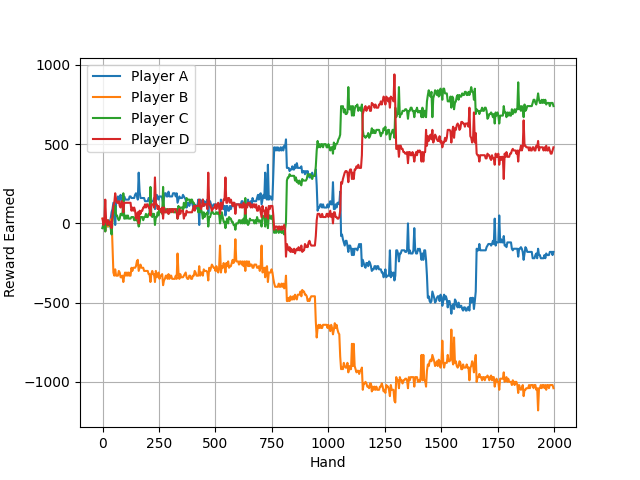
\includegraphics[size=0.75]{expampleRewardEarned.png}
    \caption{Example of Rewards Earned for 4 Players after 2000 hands}
    \label{fig:exampleCumSum}
\end{figure}
\end{center}
See Figure \ref{fig:exampleCumSum} for an example of this.\newline
This metric can be useful to get an initial idea of who is winning, but is susceptible to variance.\newline
Repeated trials often produce different results for players of equal strength.

\subsection{Win Percentage}
Firstly one can look at the overall win percentages across a sample of hands.
The win percentage can be calculated with the following formula.
\[\text{Win \%} = \frac{\# \text{ Hands Won}}{\# \text{ Hands Played}}\]
TODO example table
To achieve more detail of the agent's performance one we can further split the win percentage up into roles.
Overall there are seven roles in Schafkopf depending on the game mode, four offensive and three opposition:
\begin{itemize}
    \item Team
    \item Wenz
    \item Solo
    \item Team-Partner
    \item Team-Opposition
    \item Wenz-Opposition
    \item Solo-Opposition
\end{itemize}
For each of the seven roles we can then calculate separate win percentages with the formula above, replacing the
\textbf{Hands Won} and \textbf{Hands Played} with the respectively subset for each role.
\newline
This results for each player can then be shown in a table that allows for easy analysis of each role.
\newline
\begin{table}
\begin{tabular}{lrrrrrrr}
    \toprule
    Player & Team & Wenz & Solo & Team-Partner & Team-Opp & Wenz-Opp & Solo-
    Opp \\
    \midrule
    PlayerA & 0.506 & 0.917 & 0.864 & 0.527 & 0.505 & 0.167 & 0.226 \\
    PlayerB & 0.474 & 0.875 & 0.729 & 0.509 & 0.480 & 0.153 & 0.181 \\
    PlayerC & 0.527 & 1.000 & 0.829 & 0.518 & 0.511 & 0.194 & 0.214 \\
    PlayerD & 0.516 & 0.625 & 0.764 & 0.470 & 0.481 & 0.069 & 0.193 \\
    \bottomrule
\end{tabular}
\caption{Example of \textbf{winning percentage} for all seven roles for four players}
\label{winpercentageroles}
\end{table}
\newline
Win percentages are useful and would be sufficient if it were not for extra rewards \textit{Schneider} and
\textit{Schwarz}.
Two agents may have the same \textbf{winning percentage}, but one agent accumulates more rewards.

\subsection{Expected Value}
To address this we use \textbf{Expected Value(EV)}.
This concept is common in gambling games to express how much a certain bet or action, in our case hand, returns over
a large sample.
The formula used is the arithmetic mean:
\[ \text{EV} = \frac{1}{n} \sum_{i=1}^{n}a_{i} = \frac{a_{1} + a_{2} + ...+a_{n}}{n} \]
There are two hand metrics we can use for \textit{a\textsubscript{i}} of achieving this: \textbf{Points Scored} and
\textbf{Reward Earned}.

\subsection{Points Scored}
To calculate \textbf{EV\textsubscript{Points Scored}} of the hand sample we record the points scored and use the
above \textbf{EV} formula to calculate the metric.
\newline
\begin{table}[!h]
\centering
\begin{tabular}{cccc}
\toprule
Player A &  Player B &  Player C &  Player D\\
\midrule
32.48 & 33.71 & 27.49 & 26.32 \\
\bottomrule
\end{tabular}
\caption{EV\textsubscript{Points Scored} after 10000 games for four Players}
\label{tab:evscorestable}
\end{table}
\newline
In Table \ref{tab:evscorestable} we can see that Player A can expect to score 32.48 points per hand compared to only
the 26.32 of Player D.
In general we can say that Player A is the better player compared to Player B.
\newline
Although \textbf{EV\textsubscript{Points Scored}}certainly tells us something about playing strength, since Schafkopf
is after all a trick game, it also does not tell the whole story.
This metric scores greedy agents that only score for themselves higher than an agent that plays cooperative, even
though the cooperative agent might win more \textbf{Rewards} or even have a higher \textbf{Winning Percentage}.
\newline
It may certainly be useful but is not suitable to clearly evaluate an agent's playing strength.
Additionally one might also split up \textbf{EV\textsubscript{Points Scored}} further into the seven game role
categories, but this approach seems equally flawed.

\subsection{Rewards Earned}
To calculate \textbf{EV\textsubscript{Rewards Earned}} of the hand sample we record the rewards earned and use the
above \textbf{EV} formula to calculate the metric.
\newline
\begin{center}
\begin{table}[h!]
\begin{tabular}{cccc}
\toprule
Player A &  Player B &  Player C &  Player D\\
\midrule
2.32 &              2.92 &          -2.15 &          -3.08 \\
\bottomrule
\end{tabular}
\caption{Example of EV\textsubscript{Rewards Earned} after 10000 games for four Players}
\label{tab:EVrewardsOverall}
\end{table}
\end{center}
Table \ref{tab:EVrewardsOverall}] shows for example that Player A can expect +2.32 \textit{Reward} per hand, while
Player D can expect to lose -3.08 \textit{Reward} per hand.
To look closer at the areas that cause this we can also look again at the game roles.
\newline
\begin{center}
\begin{table}[h!]
\begin{tabular}{lrrrrrrr}
\toprule
Player &  Team &    Wenz &   Solo &  Team-Partner &  Sauspiel-Opp &  Wenz-Opp &  Solo-Opp \\
\midrule
Player A &  4.93 &   39.58 &  84.39 &          2.39 &         -0.48 &     87.89 &     -2.83 \\
Player B &  4.27 &  131.48 &  79.03 &          6.08 &          1.61 &    -47.73 &     -6.85 \\
Player C &  2.03 &  -21.07 &  13.42 &         -2.21 &         -5.46 &    -34.35 &    -80.14 \\
Player D & -2.88 &  -23.68 &   6.31 &          1.51 &         -6.18 &   -235.00 &    -98.13 \\
\bottomrule
\end{tabular}
    \caption{Example of EV\textsubscript{Rewards Earned} by game role after 10000 games for four Players}
\label{tab:EVrewardsGamemode}
\end{table}
\end{center}
\textbf{EV\textsubscript{Rewards Earned}} overcomes the previous pitfall.
It more accurately shows when agents extract value from additional rewards earned, which was not possible by simply
looking at the \textbf{Winning Percentages}, or while also taking into account the advantage of cooperative play.
\newline
\textbf{EV\textsubscript{Rewards Earned}} will be the main tool when considering playing strength.


\section{Hand Seeding \& Fairness}
To evaluate player strength we introduced seeding as it is a way to reduce variance in the game.
This concept is for example used in competitive Bridge and Scrabble[REF] as a means for fairness, since card games
often have a high degree of variance.
This variance and the low number of games played at competitive would otherwise make any competition part lottery.
\newline
For Schafkopf there are three features that define a hand:
\begin{description}
    \item [Hand distribution] The way the cards are distributed to the four seats at the table.
    \item [Relative Hand Position] Hand A sits to the right of Hand B and so on.
    \item [Initial Lead] Who starts the hand determines not just the play but also the Bidding.
\end{description}
Although fairly obvious, they act as a minimal and sufficient way of describing the initial state of a game.
In order to control for these, a seeding mechanism was introduced that can be called when initialising the game
environment.
This alone however is not enough to reduce the variance between four players, as it only allows to control the
seeding between two tables of players.
\newline
If we imagine a tournament in which the 12 hands (or three rounds) are played at Table A and Table B, so that A and B
receive the same hands, in order to find the best player among both tables.
It might happen that the majority of hands are favourable for Seat 1, and the player in that seat wins by a big margin.
The same or similar would happen on Table B and no one is the wiser to who is the strongest player.
\newline
To get around this, we introduced "Fair tournaments" that play each seed four times, each player gets to play the hand
from every seat once.
[IMAGE of rotation]
[CODE Fair tournament]
This way, player strength can be evaluated to a good degree, since good cards cancel out and marginal
advantages in playing strength are rewarded.
Agent 1 might score with accurate play for the same seed more reward the Agent 2 by receiving an extra reward for
Schneider.
\newline
As a last point, it should be said that there is still some variance due to the players.
Firstly most players (and also agents used here) do not play completely deterministic, thus sometimes they make
incorrect decision, and this being an imperfect information game, two identical seeds will not produce the same game.
\newline
On the other hand, the order the players sit at the table may also have some effect.
Player A,B,C and D, all of differing strength, can have [FORMULA]4! seating arrangements that would each have to be
played four times.
\[\text{Hands per Seed} = 4! * 4 = 96\]
96 hands per seed would be more fair, but seems in the scope of this work unnecessary and due to the above
potentially still not sufficient.

In order to test our networks we designed baseline agents to play against, to measure playing strength.
The agents all use same \textit{makebid()} method to establish an even playing field, on which we can compare pure
playing strength.
Each agent's strategy will be briefly explained and statistics from a fair tournament, which is played between four
instances of the respective player,will be given to get an idea of their perfomance.
\newline
See Table \ref{tab:baselinevs} for an inbetween comparison of three baseline agents, each playing 10000 hands
against each other.
\begin{table}[!h]
    \centering
    \begin{tabular}{lccc}
        \toprule
        Player    & Random & Greedy & Heuristic \\
        \midrule
        Random    & -      & -4.55  & -5.48     \\
        Greedy    & 4.55   & -      & -1.35     \\
        Heuristic & 5.48   & 1.35   & -         \\
        \bottomrule
    \end{tabular}
    \caption{Baseline agent tournament that shows the order of strenght in accending order: Random, Greedy, Heuristic}
    \label{tab:baselinevs}
\end{table}


\section{Static Bidding}
Table \ref{tab:distributionBidding} shows the distribution of contracts.
We can see that the majority of hands are Team contracts, whilst the remaining 15\% of games are envenly distributed
over the remaining Solo contracts.\\
The bidding heuristic used here is by no means expert play but overall reasonable for what we are trying to achieve.
Human players are likely to play a somewhat higher percentage of Solo games, although that frequency is heavily
affected of one's one playing strength, and ideally varied according to one's opponents abilities.
To find a balance between win rate and winning frequency is major part in contract card games such as Bridge and
Schafkopf.
\begin{table}[!h]
    \centering
    \begin{tabular}{lc}
        \toprule
        Contract    & Distribution \\
        \midrule
        Team        & 85,3         \\
        Wenz        & 6,6          \\
        Colour-Solo & 8,1          \\
        No Game     & 0,0          \\
        \bottomrule
    \end{tabular}
    \caption{Distribution of contracts}
    \label{tab:distributionBidding}
\end{table}


\section{Baseline Agents}
The following table shows the baseline comparison between the three baseline agents, each playing 10000 hands against
one another.

\subsection{Random Agent}
The Random agent plays like the name suggests a random valid card.
It makes no use of the passed games state, has no understanding of team composition and performs expectantly bad.
This strategy is terrible for all contracts, although some hands can still be played near optimal, due to holding good
cards, having competent teammates, or having little choice.
\begin{table}[!h]
    \centering
    \begin{tabular}{ccccccc}
        \toprule
        Team  & Wenz  & Solo  & Team-Partner & Sauspiel-Opp & Wenz-Opp & Solo-Opp \\
        \midrule
        0.616 & 0.539 & 0.843 & 0.616        & 0.384        & 0.461    & 0.157    \\
        \bottomrule
    \end{tabular}
    \caption{Average win rates of Random agent against itself over 10000 hands}
    \label{tab:winratesRan}
\end{table}

\subsection{Greedy Agent}
The Greedy agent will always try to win every trick possible.
It understands trumps, tricking, point values, but has no understanding of team composition.
When he has the lead it chooses to play the highest rank that is not trump, or the highest trump if it only holds trump.
When not in the lead it will test if it can beat the cards in the current trick, even if one of his partner currently
is the trick winner.
If it holds more than one winning card it will choose the card with the highest point value.
Vice Versa if it holds no winning card it will choose the lowest point value card, if possible not trump, even if
that means playing an Ace.\\
In summary,Greedy agent values winning tricks and not giving up trump if possible.
This strategy can certainly be viable for Solo contracts where itself is the bid winner, but will fail when it is
part of the opposition, because trumps are sparse and over-tricking teammates is major error.
For team contracts it [LOOK at stats, might be ok for]
\begin{table}[!h]
    \centering
    \begin{tabular}{ccccccc}
        \toprule
        Team  & Wenz  & Solo  & Team-Partner & Sauspiel-Opp & Wenz-Opp & Solo-Opp \\
        \midrule
        0.604 & 0.646 & 0.757 & 0.604        & 0.396        & 0.354    & 0.243    \\
        \bottomrule
    \end{tabular}
    \caption{Average win rates of Greedy agent against itself over 10000 hands}
    \label{tab:winratesGre}
\end{table}

\subsection{Heuristic Agent}
The Heuristic agent is a lot more nuanced than the above agents.
It employs a separate strategy for each of seven game positions and uses the game state to infer the team composition
,if possible, and uses the strategies from \ref{basicstrategy} to some extent.\\
Furthermore it understands everything Greedy agent knows, about points, trump and tricking.
Its limitations are its use of the trick history, which is only used when it plays in the offensive or team partner
role to infer how many trumps are still with the others, but misses strategies, such as leading a suit where a
teammate is known to be, or similar.
The decision process is mostly deterministic, but there are situations where two cards are equally playable and one is
randomly chosen.\\
Heuristic agent is certainly a decent opponent that follows good practice play a novice might bring to the table.
\begin{table}[!h]
    \centering
    \begin{tabular}{ccccccc}
        \toprule
        Team  & Wenz  & Solo  & Team-Partner & Sauspiel-Opp & Wenz-Opp & Solo-Opp \\
        \midrule
        0.485 & 0.588 & 0.695 & 0.485        & 0.515        & 0.412    & 0.305    \\
        \bottomrule
    \end{tabular}
    \caption{Average win rates of Heuristic agent against itself over 10000 hands}
    \label{tab:win ratesHeu}
\end{table}
    \chapter{Player Agents}
\section{Base Player Class}
\section{Static Bidding}
\section{Random Agent}
\section{Heuristic}
\section{Random Sample}
\section{Smart Sample}
\section{RL}
    \chapter{Results}
In this chapter we will present our overall results, by showing our training data, the hyper-parameters used, and
explain what worked and did not work.
Afterwards we will evaluate the best models and present our evaluation data.
\section{Training Experiments}
In \textbf{PPO} there are a number of hyper parameters that can be tweaked to achieve convergence.
An overview of the general parameters used can be seen in Table \ref{tab:hyper}.
\begin{table}[!ht]
    \begin{tabularx}{\linewidth}{lllX}
        \toprule
        Name & Value Used & Method & Description
        \\
        \midrule
        Hands Played & {[}500,15000{]} & Varied & The number of data points that go into each
        episode. Hands * 4 * 8 \\
        Batch Size & 80\% of the data & Fixed & The absolute size is dependent on the number of
        hands played \\
        Epochs & {[}8,16{]} & Varied & Number of Epochs(K) per episode
        \\
        Learning Rate & 0.0002 & Fixed & Used for Adams Optimiser
        \\
        Learning Rate Gamma & 0.3 & Fixed & Learning rate
        \\
        Clipping Range & 0.2 & Fixed & Clipping range to mange the clip the incremental
        change \\
        Discount Factor & 0.99 & Fixed & Used to calculate Discounted Rewards for
        Non-Terminal steps \\
        Value Function Coefficient & 0.5 & Fixed & (c1) Coefficent that allows computation of a
        comibined loss for actor-critic \\
        Entropy Coefficient        & 0.005            & Fixed  & (c2) Stops the model from early convergence
        \\
        Optimiser Weight Decay     & 1e-5             & Fixed  & Weight decay used in Adams Optimiser
        \\
        \bottomrule
    \end{tabularx}
    \caption{Hyperparameters used throughout the training.}
    \label{tab:hyper}
\end{table}

\subsection{CompleteRL}
For CompleteRL we experimented a fair bit with batch different values of the amount of hands played and it quickly
became apparent that CompleteRL was highly dependent on that number to be large.\\
Anything under 10000 (batch size = 256000,K=16) would simply not converge, and the distribution entropy was hovering
around 0.8, which means that the probabilities of actions effectively represented that of the Random agent.\\
Potential adjustment of the hyper-paramaters might solve this, but we doubt that.
\newline
One experiment that was successful was running 150000 hands(batch size=300000,K=16) over 80 steps.
Fig. \ref{fig:15comp} shows the achieved training progress.
\begin{figure}[!ht]
    \centering
    \subfloat[][Policy Loss]{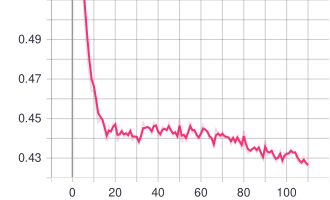
\includegraphics[width=.4\textwidth]{15com/Loss_policy_loss}}\quad
    \subfloat[][Entropy]{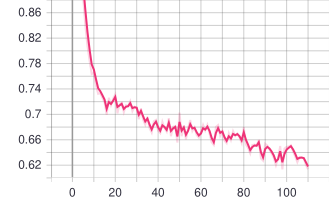
\includegraphics[width=.4\textwidth]{15com/Loss_value_loss}}\\
    \subfloat[][Value Loss]{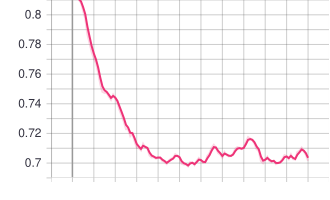
\includegraphics[width=.4\textwidth]{15com/Loss_entropy}}\quad
    \subfloat[][Explained Variance]{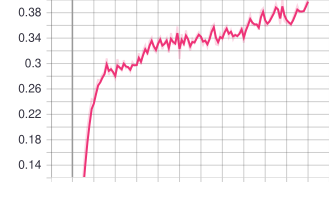
\includegraphics[width=.4\textwidth]{15com/Loss_avg_explained_var}}
    \caption{CompleteRL with 15000 hands per episode and K=16}
    \label{fig:15comp}
\end{figure}

\subsection{SeperatedRL}
For the training of \textbf{SepereratedRL} we experimented with smaller networks as our intuiton was that since we
train each gamemode individually less data might suffice.
CompleteRL for example only sees around 6\% Colo-Solos per episode, so the network a with 15000 hands might only sees
600 hands, that might get lost in the noise of all the other hands.
We therefore trained SeperatedRL with only 500 hands per episode (batch size =16000,K=8) and still managed to
reach convergence over 100 episodes.
\begin{figure}[!h]
    \centering
    \subfloat[][Policy Loss]{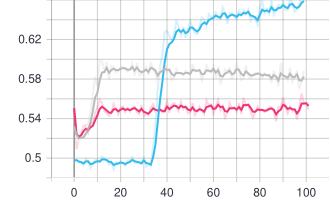
\includegraphics[width=.4\textwidth]{500sad/Loss_policy_loss}}\quad
    \subfloat[][Entropy]{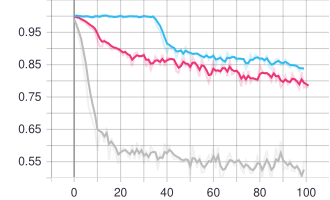
\includegraphics[width=.4\textwidth]{500sad/Loss_value_loss}}\\
    \subfloat[][Value Loss]{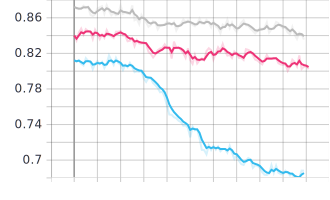
\includegraphics[width=.4\textwidth]{500sad/Loss_entropy}}\quad
    \subfloat[][Explained Variance]{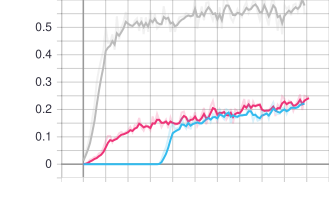
\includegraphics[width=.4\textwidth]{500sad/Loss_avg_explained_var}}
    \caption{SeperateRL with 500 hands per episode and K=8.(blue=Team,red=Solo,grey=Wenz)}
    \label{fig:500sep}
\end{figure}


\section{Results against Baselines}
We now show the data of the latest episode in play against our baselines.
For each agent we played 10000 hands in a fair tournament that controls for the seeding, to ensure minimal variance.

\subsection{CompleteRL}
When we look at Table \ref{tab:evCompleteRL} we can see that CompleteRL was only able to beat the Random agent,
convincingly, while losing against the other two by a good margin.\\
\newline
\begin{table}[!h]
    \centering
    \begin{tabular}{lccc}
        \toprule
        Player     & Random & Greedy & Heuristic \\
        \midrule
        CompleteRL & 2.11   & -1.63  & -2.65     \\
        \bottomrule
    \end{tabular}
    \caption{EV Overall: CompleteRL versus the baselines}
    \label{tab:evCompleteRL}
\end{table}

\begin{table}
    \begin{tabular}{lrrrrrrr}
        \toprule
        {}          & Team & Wenz & Solo & Team-Partner & Sauspiel-Opp & Wenz-Opp & Solo-Opp \\
        \midrule
        CompleteRL1 & 0.75 & 0.56 & 0.72 & 0.74         & 0.20         & 0.29     & 0.16     \\
        heu1        & 0.79 & 0.78 & 0.89 & 0.80         & 0.25         & 0.37     & 0.21     \\
        CompleteRL2 & 0.75 & 0.54 & 0.75 & 0.74         & 0.20         & 0.29     & 0.17     \\
        heu2        & 0.79 & 0.79 & 0.89 & 0.80         & 0.25         & 0.37     & 0.21     \\
        \bottomrule
    \end{tabular}
    \caption{Winrates: CompleteRL against Heuristic agent}
    \label{tab:heuCom}
\end{table}

\begin{table}
    \begin{tabular}{lrrrrrrr}
        \toprule
        {}          & Team & Wenz & Solo & Team-Partner & Sauspiel-Opp & Wenz-Opp & Solo-Opp \\
        \midrule
        CompleteRL1 & 0.76 & 0.56 & 0.85 & 0.76         & 0.18         & 0.33     & 0.12     \\
        Greedy1     & 0.81 & 0.72 & 0.89 & 0.82         & 0.24         & 0.39     & 0.13     \\
        CompleteRL2 & 0.76 & 0.56 & 0.85 & 0.76         & 0.18         & 0.33     & 0.12     \\
        Greedy2     & 0.81 & 0.72 & 0.89 & 0.82         & 0.24         & 0.39     & 0.13     \\
        \bottomrule
    \end{tabular}
    \caption{Winrates: CompleteRL against Greedy agent}
    \label{tab:greedyRL}
\end{table}

\begin{table}
    \begin{tabular}{lrrrrrrr}
        \toprule
        {}          & Team & Wenz & Solo & Team-Partner & Sauspiel-Opp & Wenz-Opp & Solo-Opp \\
        \midrule
        CompleteRL1 & 0.81 & 0.75 & 0.92 & 0.78         & 0.24         & 0.37     & 0.11     \\
        Random1     & 0.73 & 0.55 & 0.85 & 0.79         & 0.20         & 0.30     & 0.09     \\
        CompleteRL2 & 0.81 & 0.77 & 0.95 & 0.77         & 0.23         & 0.37     & 0.13     \\
        Random2     & 0.77 & 0.59 & 0.86 & 0.78         & 0.21         & 0.31     & 0.10     \\
        \bottomrule
    \end{tabular}
    \caption{Winrates: CompleteRL against Random agent}
    \label{tab:rancom}
\end{table}

\subsection{SeperatedRL}
\begin{table}[!h]
    \centering
    \begin{tabular}{lccc}
        \toprule
        Player     & Random & Greedy & Heuristic \\
        \midrule
        CompleteRL & 1.89   & -4.02  & -4.34     \\
        \bottomrule
    \end{tabular}
    \caption{EV Overall: CompleteRL versus the baselines}
    \label{tab:evSeperateRL}
\end{table}

\begin{table}
    \begin{tabular}{lrrrrrrr}
        \toprule
        {}          & Team & Wenz & Solo & Team-Partmer & Sauspiel-Opp & Wenz-Opp & Solo-Opp \\
        \midrule
        SeperateRL1 & 0.73 & 0.44 & 0.68 & 0.74         & 0.21         & 0.29     & 0.15     \\
        Heuristic1  & 0.80 & 0.86 & 0.92 & 0.79         & 0.26         & 0.43     & 0.23     \\
        SeperateRL2 & 0.74 & 0.41 & 0.69 & 0.74         & 0.21         & 0.28     & 0.16     \\
        Heuristic2  & 0.80 & 0.86 & 0.93 & 0.79         & 0.26         & 0.43     & 0.24     \\
        \bottomrule
    \end{tabular}

    \caption{Winrates: SeperateRL against Heuristic agent}
    \label{tab:heusep}
\end{table}

\begin{table}
    \begin{tabular}{lrrrrrrr}
        \toprule
        {}          & Team & Wenz & Solo & Team-Partner & Sauspiel-Opp & Wenz-Opp & Solo-Opp \\
        \midrule
        SeperateRL1 & 0.73 & 0.54 & 0.71 & 0.75         & 0.19         & 0.26     & 0.16     \\
        Greedy1     & 0.82 & 0.84 & 0.91 & 0.80         & 0.26         & 0.36     & 0.22     \\
        SeperateRL2 & 0.73 & 0.54 & 0.71 & 0.75         & 0.19         & 0.26     & 0.16     \\
        Greedy2     & 0.82 & 0.84 & 0.91 & 0.80         & 0.26         & 0.36     & 0.22     \\
        \bottomrule
    \end{tabular}
    \caption{Winrates: SeperateRL against Greedy agent}
    \label{tab:greedysep}
\end{table}

\begin{table}
    \begin{tabular}{lrrrrrrr}
        \toprule
        {}          & Team & Wenz & Solo & Team-Partner & Sauspiel-Opp & Wenz-Opp & Solo-Opp \\
        \midrule
        SeperateRL1 & 0.80 & 0.66 & 0.86 & 0.79         & 0.24         & 0.45     & 0.16     \\
        Random1     & 0.77 & 0.49 & 0.80 & 0.76         & 0.21         & 0.39     & 0.14     \\
        SeperateRL2 & 0.78 & 0.73 & 0.88 & 0.80         & 0.23         & 0.47     & 0.17     \\
        Random2     & 0.76 & 0.42 & 0.84 & 0.76         & 0.20         & 0.37     & 0.15     \\
        \bottomrule
    \end{tabular}
    \caption{Winrates: SeperateRL against Random agent}
    \label{tab:ransep}
\end{table}

\subsection{CompleteRL against SeperateRL}
At last we pitted our two RL agents against each other.
The results are little surprising after the previous play versus the baselines.\\
More surprising is the fact, that SeperateRL is not performing well in at least the Solo contracts, which it should
have an advantage in terms of seen games.
\begin{table}[!h]
    \centering
    \begin{tabular}{cccc}
        \toprule
        SeperateRL1 & ComleteRL1 & SeperateRL2 & ComleteRL2 \\\\
        \midrule
        -2.17 & 2.17 & -2.17 & 2.17 \\\\
        \bottomrule
    \end{tabular}
    \caption{EV Overall: CompleteRL against SeperatedRL}
    \label{tab:comRlwin}
\end{table}

\begin{table}
    \begin{tabular}{lrrrrrrr}
        \toprule
        {}          & Team & Wenz  & Solo  & Team-Partner & Sauspiel-Opp & Wenz-Opp & Solo-Opp \\
        \midrule
        SeperateRL1 & 2.32 & 8.90  & 40.18 & 2.37         & -4.00        & -15.21   & -21.58   \\
        CompleteRL1 & 4.03 & 38.46 & 46.53 & 3.97         & -2.35        & -0.57    & -7.33    \\
        SeperateRL2 & 2.32 & 8.90  & 40.18 & 2.37         & -4.00        & -15.21   & -21.58   \\
        CompleteRL2 & 4.03 & 38.46 & 46.53 & 3.97         & -2.35        & -0.57    & -7.33    \\
        \bottomrule
    \end{tabular}
    \begin{tabular}{lrrrrrrr}
        \toprule
        {}          & Team & Wenz & Solo & Team-Partner & Sauspiel-Opp & Wenz-Opp & Solo-Opp \\
        \midrule
        SeperateRL1 & 0.75 & 0.66 & 0.84 & 0.78         & 0.20         & 0.23     & 0.09     \\
        CompleteRL1 & 0.82 & 0.83 & 0.94 & 0.79         & 0.23         & 0.28     & 0.12     \\
        SeperateRL2 & 0.75 & 0.66 & 0.84 & 0.78         & 0.20         & 0.23     & 0.09     \\
        CompleteRL2 & 0.82 & 0.83 & 0.94 & 0.79         & 0.23         & 0.28     & 0.12     \\
        \bottomrule
    \end{tabular}
    \caption{EV: CompleteRL against SeperatedRL}
    \label{tab:comRlev}
\end{table}

\begin{figure}[!h]
    \centering
    \includegraphics[width=\textwicumsums.png.png}
\caption{Points after 10000 hands for ComleteRL vs SeperateRL}
\label{fig:cumsums}
\end{figure}
%
% =================================================================================================
% place your appendix here
% -------------------------------------------------------------------------------------------------
%
    \appendix
    % -------------------------------------------------------------------------------------------------
%      MDSG Latex Framework
%      ============================================================================================
%      File:                  appendix.tex
%      Author(s):             Michael Duerr
%      Version:               1
%      Creation Date:         30. Mai 2010
%      Creation Date:         30. Mai 2010
%
%      Notes:                 - Place your appendix here
%                             - Use the same commands (`chapter', `section', ...) as in main text
% -------------------------------------------------------------------------------------------------
%
\chapter{Beispiel Anhang}
\small{
\begin{verbatim}
/*
* This code serves the initialization of an auxiliary probability array.
* The array holds at each position a pre-calculated probability for the index
* of that position. The probability reflects the Zipf-distribution for the
* corresponding indexes
*/
Set zipfExponent to 1.4
Set sum to 0
Set maxInteger to 65535
FOR i = 0 to maxInteger
probArray[i] = 1/pow(i + 1, zipfExponent)
Set sum = sum + probArray[i]
END FOR
FOR i = 0 to maxInteger
Set probArray[i] = probArray[i]/sum
END FOR
FOR i = 1 to maxInteger
Set probArray[i] = probArray[i] + probArray[i] = probArray[i-1]
END FOR

/*
* This code gets called in case a Zipf-distributed number is required. It
* iterates over the probability array until the chosen random number v
* is less than the value stored at the current array position i. The value of
* the array position will be returned as the calculated Zipf-distributed
* number
*/
Set v to a random number between 0 and 1
FOR i = 0 to maxInteger
IF v < probArray[i] THEN
RETURN i
END IF
END FOR
RETURN 0

\end{verbatim}
}

    % further appendix
%
% =================================================================================================
% comment \listoffigures and/or \listoftables if not wanted
% -------------------------------------------------------------------------------------------------
%
    \backmatter
    \listoffigures                                % list of figures (uncomment if wanted)
    \listoftables                                 % list of tables (uncomment if wanted)
    \lstlistoflistings                            % list of listings (uncomment if wanted)
%
% =================================================================================================
% place your bibliography here
% -------------------------------------------------------------------------------------------------
%
    \begin{spacing}{0.9}                          % save some space
        %\bibliographystyle{geralpha}               % for german thesis
        \bibliographystyle{alpha}                 % for english thesis
        \bibliography{bibliography}                % the location of bib file
    \end{spacing}
\end{document}
%
% =================================================================================================
% end of document
% -------------------------------------------------------------------------------------------------
%